\documentclass[10pt, aspectratio=169]{beamer}

\usepackage[T1]{fontenc}
\usepackage{amsmath, bm}
\usepackage{multicol}
\usepackage{booktabs}
\usepackage{multimedia}
\usepackage{caption}
\usepackage{xcolor}
\usepackage{amssymb}
\usepackage{tensor}
\usepackage{hyperref}
\usetheme{Madrid}


\author{Christos Mermigkas}
\title{Computational Methods on Black Hole Imaging}
\subtitle{Relativistic Ray Tracing via Automatic Differentiation and Geometric Integration}
\institute{Aristotle University of Thessaloniki \\ Computational Physics MSc}
\date{October 2026}


\begin{document}
	
	\begin{frame}
		\titlepage
	\end{frame}
	
	\begin{frame}{Outline}
		\tableofcontents
	\end{frame}
	
	\section{Motivation}
	
	\begin{frame}{From Gargantua to M87*: The Science of Black Hole Imaging}
		\begin{itemize}
			\item \textbf{2014:} The movie \textit{Interstellar} showed the world a realistic black hole ``Gargantua'' - computed using actual General Relativity equations.
			\item \textbf{2019:} The Event Horizon Telescope (EHT) revealed the first real image of a black hole (M87*).
			\item \textbf{The common thread:} Both rely on \textbf{relativistic ray tracing} - tracing light paths through curved spacetime.
		\end{itemize}
		\vspace{0.3cm}
		\begin{block}{The Central Question}
			\textit{What would an observer actually see when looking at a black hole?} \\[0.2cm]
			Answering this requires solving the geodesic equation with \textbf{machine-precision accuracy} in a chaotic, strong-field environment.
		\end{block}
	\end{frame}
	
	\begin{frame}{The Computational Challenge}
		\begin{itemize}
			\item \textbf{Goal:} Trace millions of photon trajectories backwards from the observer to the source.
			\item \textbf{Problem:} Near the photon sphere, trajectories are \textbf{chaotic} (Lyapunov instability).
			\item Tiny numerical errors $\rightarrow$ exponential divergence $\rightarrow$ unphysical results.
			\item \textbf{Requirement:} Machine-precision accuracy over long integration times.
		\end{itemize}
		\vspace{0.3cm}
		\begin{block}{Our Solution}
			A metric-agnostic framework in Julia combining:
			\begin{enumerate}
				\item Automatic Differentiation
				\item Manifold Projection
			\end{enumerate}
		\end{block}
	\end{frame}

	\section{Computational Methods}
	
	\subsection{The Geodesic Equation}
	
	\begin{frame}{What We Compute: The Geodesic Equation}
		\begin{itemize}
			\item \textbf{Physical problem:} Find the path $x^\mu(\lambda)$ of a photon in curved spacetime.
			\item \textbf{The equation:}
			\begin{equation}
				\ddot{x}^\mu + \tensor{\Gamma}{^\mu_{\alpha\beta}} \dot{x}^\alpha \dot{x}^\beta = 0
			\end{equation}
			\item where $\tensor{\Gamma}{^\mu_{\alpha\beta}}$ are the Christoffel symbols:
			\begin{equation}
				\tensor{\Gamma}{^\mu_{\alpha\beta}} = \frac{1}{2} g^{\mu\sigma} \left( \partial_\alpha g_{\beta\sigma} + \partial_\beta g_{\alpha\sigma} - \partial_\sigma g_{\alpha\beta} \right)
			\end{equation}
			\item \textbf{The bottleneck:} We need $\partial_\sigma g_{\mu\nu}$ - the derivatives of the metric tensor.
		\end{itemize}
	\end{frame}
	
	\subsection{Method 1: Automatic Differentiation}
	
	\begin{frame}{AD: Why Finite Differences Fail}
		\begin{itemize}
			\item \textbf{Traditional approach:} Finite Differences (FD)
			\begin{equation}
				\partial_\sigma g_{\mu\nu} \approx \frac{g_{\mu\nu}(x+h) - g_{\mu\nu}(x-h)}{2h}
			\end{equation}
			\item \textbf{Two competing errors:}
			\begin{itemize}
				\item \textbf{Truncation error:} $\mathcal{O}(h^2)$ - decreases as $h \to 0$
				\item \textbf{Round-off error:} $\mathcal{O}(\epsilon_{\text{mach}}/h)$ - increases as $h \to 0$
			\end{itemize}
			\item \textbf{Result:} U-shaped error curve.
		\end{itemize}
	\end{frame}
	
	\begin{frame}{AD: How Dual Numbers Work}
		\begin{itemize}
			\item \textbf{Idea:} Extend real numbers with an infinitesimal $\epsilon$ where $\epsilon^2 = 0$.
			\item \textbf{Dual number:} $x = a + b\epsilon$ (value $a$, derivative $b$).
			\item \textbf{Key insight:} If we evaluate $f(x + 1\cdot\epsilon)$, the Taylor expansion gives:
			\begin{equation}
				f(x + \epsilon) = f(x) + f'(x)\underbrace{\epsilon}_{\text{derivative part}} + \frac{1}{2}f''(x)\underbrace{\epsilon^2}_{=0} + \dots = f(x) + f'(x)\epsilon
			\end{equation}
			\item \textbf{How it works in practice:}
			\begin{enumerate}
				\item Start with input $x = a + 1\cdot\epsilon$ (value $a$, derivative $1$).
				\item Apply operations (add, multiply, sin, exp, etc.) using dual number rules.
				\item Each operation propagates both value and derivative.
				\item Final result: $f(a) + f'(a)\epsilon$ --- the coefficient of $\epsilon$ is the exact derivative!
			\end{enumerate}
			\item \textbf{Chain rule:} Applied algebraically to every operation:
			\begin{itemize}
				\item $(a + b\epsilon) + (c + d\epsilon) = (a+c) + (b+d)\epsilon$
				\item $(a + b\epsilon) \cdot (c + d\epsilon) = ac + (ad+bc)\epsilon$
			\end{itemize}
			\item \textbf{Result:} \textbf{Exact} derivatives to machine precision ($\sim 10^{-16}$).
		\end{itemize}
	\end{frame}
	
	\begin{frame}{AD: Example with Chain Rule --- $f(x) = x \cdot \sin(x)$ at $x=\pi/2$}
		\begin{itemize}
			\item \textbf{Input:} $x = \frac{\pi}{2} + 1\cdot\epsilon$.
			\item \textbf{Step 1:} Compute $\sin(x)$ using dual sine rule $\sin(a+b\epsilon) = \sin(a) + \cos(a)\,b\epsilon$:
			\begin{equation}
				\sin\!\left(\tfrac{\pi}{2} + \epsilon\right) = \sin\!\left(\tfrac{\pi}{2}\right) + \cos\!\left(\tfrac{\pi}{2}\right)\epsilon = 1 + 0\cdot\epsilon = 1
			\end{equation}
			\item \textbf{Step 2:} Multiply $x \cdot \sin(x)$:
			\begin{align*}
				\left(\tfrac{\pi}{2} + 1\epsilon\right) \cdot \left(1 + 0\epsilon\right) &= \tfrac{\pi}{2}\cdot 1 + \left(\tfrac{\pi}{2}\cdot 0 + 1\cdot 1\right)\epsilon \\
				&= \tfrac{\pi}{2} + 1\cdot\epsilon
			\end{align*}
			\item \textbf{Read off:} $f(\pi/2) = \pi/2$, \quad $f'(\pi/2) = 1$ \quad $\checkmark$
		\end{itemize}
		\vspace{0.2cm}
		\begin{block}{Key takeaway}
			Every elementary function (sin, cos, exp, log, \dots) has a dual-number extension. By chaining them, the computer builds the full derivative of \emph{any} composite function - exactly, with no truncation error.
		\end{block}
	\end{frame}
	
	\begin{frame}{AD: What, Why, How}
		\begin{itemize}
			\item \textbf{What we compute:} $\partial_\sigma g_{\mu\nu}$ and $\tensor{\Gamma}{^\mu_{\alpha\beta}}$ automatically.
			\item \textbf{Why:} To feed the geodesic equation with exact accelerations.
			\item \textbf{How:} Julia's ForwardDiff package propagates dual numbers through the metric function.
			\vspace{0.3cm}
			\begin{center}
				\begin{minipage}{0.7\textwidth}
					\begin{block}{Bonus!}
						\small Metric-agnostic, works for any spacetime without manual derivation.
					\end{block}
				\end{minipage}
			\end{center}
		\end{itemize}
	\end{frame}
	
	\begin{frame}{AD: Test Result --- FD vs AD}
		\begin{figure}
			\centering
			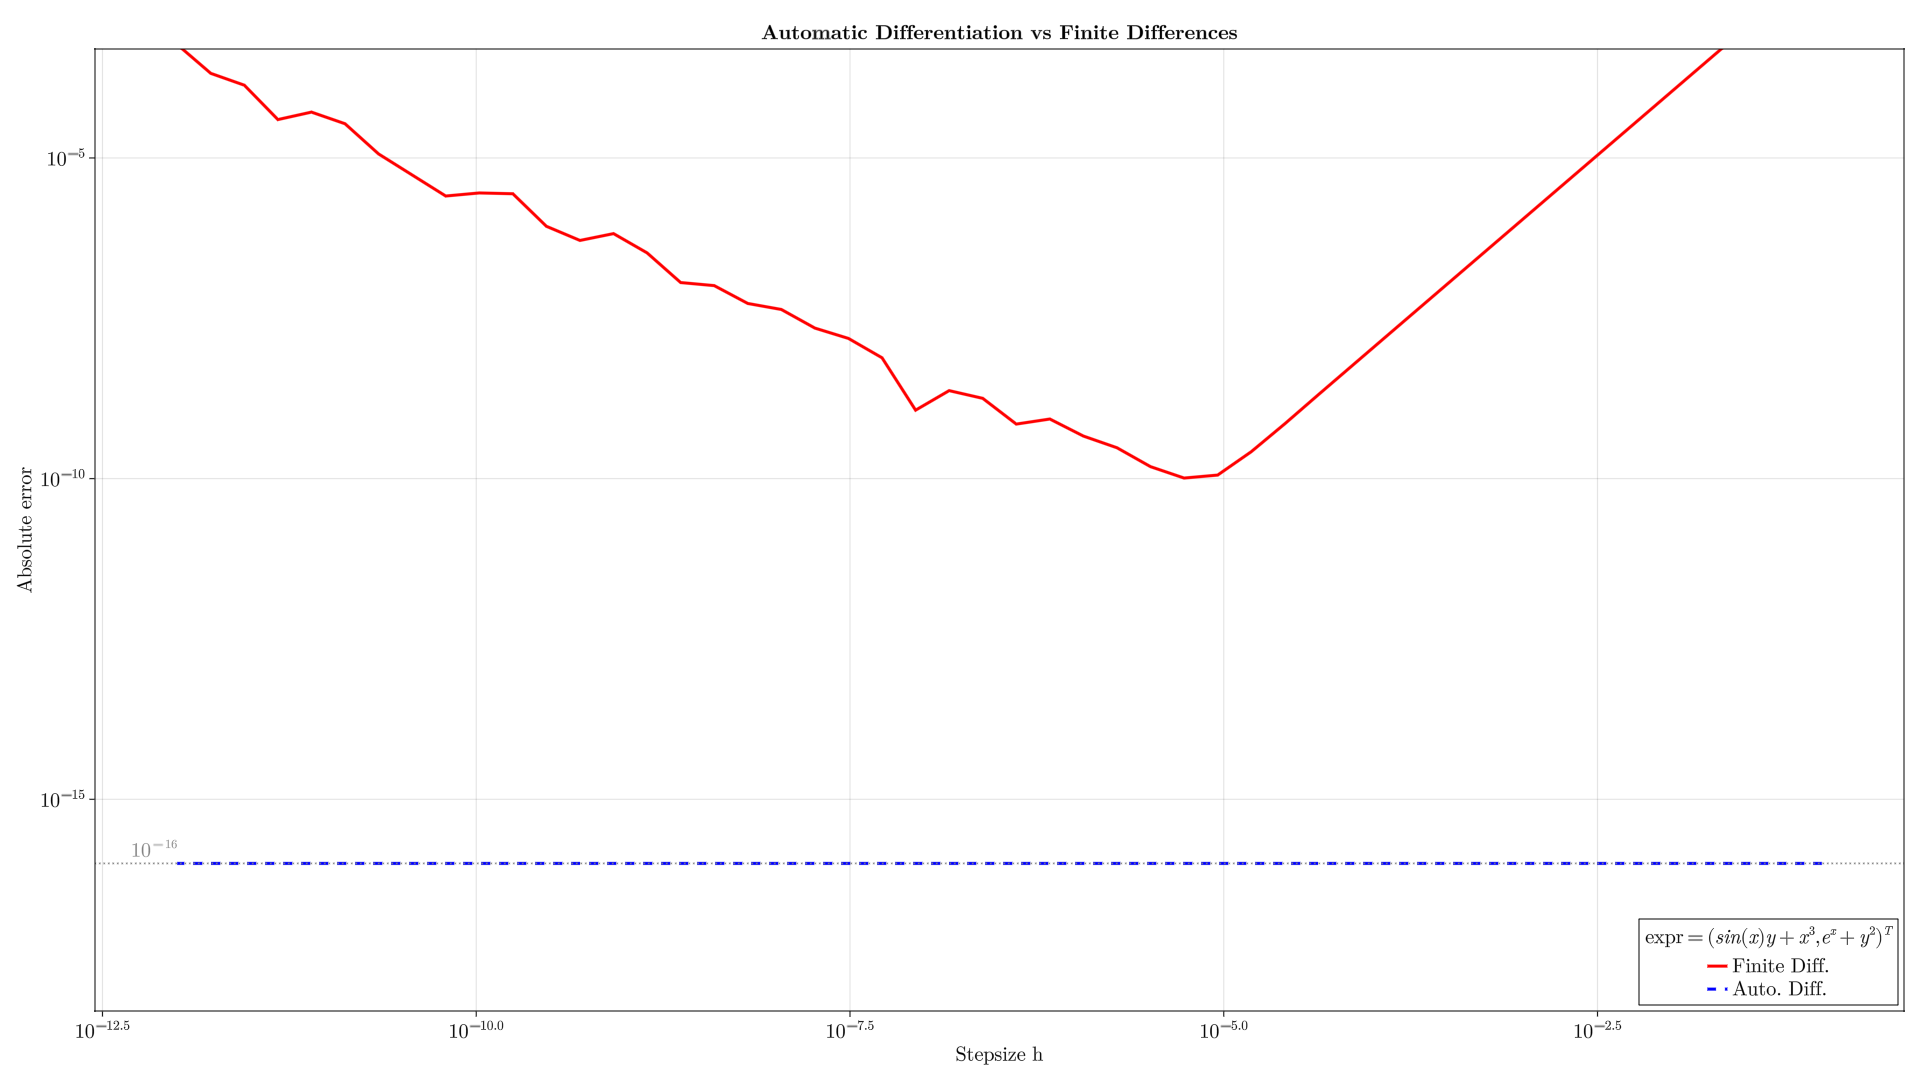
\includegraphics[width=0.85\textwidth]{figures/FDvsAD.png}
		\end{figure}
	\end{frame}
	
	\subsection{Method 2: Manifold Projection}
	
	\begin{frame}{The Problem: Invariant Drift}
		\begin{itemize}
			\item \textbf{What happens:} Standard Runge-Kutta accumulates floating-point errors.
			\item \textbf{Physical constraints (the manifold $\mathcal{N}$):}
			\begin{enumerate}
				\item \textbf{Null condition:} $g_1(\bm{y}) \equiv g_{\mu\nu} u^\mu u^\nu = 0$
				\item \textbf{Energy:} $g_2(\bm{y}) \equiv E - E_0 = 0$
				\item \textbf{Angular momentum:} $g_3(\bm{y}) \equiv L_z - L_{z0} = 0$
			\end{enumerate}
			\item \textbf{Consequence:} The numerical solution $\tilde{\bm{y}}$ drifts off $\mathcal{N}$.
			\item Near the photon sphere $\rightarrow$ exponential divergence.
		\end{itemize}
	\end{frame}
	
	\begin{frame}{Manifold Projection: The Mathematical Idea}
		\begin{itemize}
			\item \textbf{Goal:} After each RK step, project $\tilde{\bm{y}}$ back onto $\mathcal{N}$.
			\item \textbf{Method:} Lagrange multipliers - minimize distance subject to constraints:
			\begin{equation}
				\mathcal{S}(\bm{y}^*, \bm{\lambda}) = \frac{1}{2} \|\bm{y}^* - \tilde{\bm{y}}\|^2 + \bm{\lambda}^T \bm{g}(\bm{y}^*)
			\end{equation}
			\item \textbf{Solution:}
			\begin{equation}
				\bm{y}^* = \tilde{\bm{y}} - \bm{J}^T \bm{\lambda}, \quad \bm{J} = \frac{\partial \bm{g}}{\partial \bm{y}}
			\end{equation}
			\item \textbf{Key property:} Correction is \textit{\textbf{orthogonal}} to the physical flow - no artificial damping.
		\end{itemize}
	\end{frame}
	
	\begin{frame}{Manifold Projection: Newton-Raphson Solver}
		\begin{itemize}
			\item \textbf{We need to solve:} $\bm{g}(\bm{y}^*) = 0$ for $\bm{\lambda}$.
			\item \textbf{Newton-Raphson iteration:}
			\begin{equation}
				\bm{G} \, \Delta \bm{\lambda}^{(k)} = -\bm{g}(\bm{y}^{(k)}), \quad \bm{G} = \bm{J}\bm{J}^T
			\end{equation}
			\item \textbf{Algorithm:}
			\begin{enumerate}
				\item Initialize $\bm{\lambda}^{(0)} = 0$, $\bm{y}^{(0)} = \tilde{\bm{y}}$
				\item Compute $\bm{J}$ using AD (exact Jacobian!)
				\item Iterate until $\|\Delta \bm{\lambda}\| \leq tol$
			\end{enumerate}
			\item \textbf{Quadratic convergence:} Correct digits double each iteration.
		\end{itemize}
	\end{frame}
	
	\begin{frame}{Manifold Projection: Interactive Demo}
		\begin{itemize}
			\item \textbf{Test:} Harmonic oscillator $\dot{x}=y$, $\dot{y}=-x$ (analytical: circle).
		\end{itemize}
		\vspace{0.3cm}
		\begin{center}
			\href{run:figures/manifold_projection_demo.mp4}{
				\fbox{
					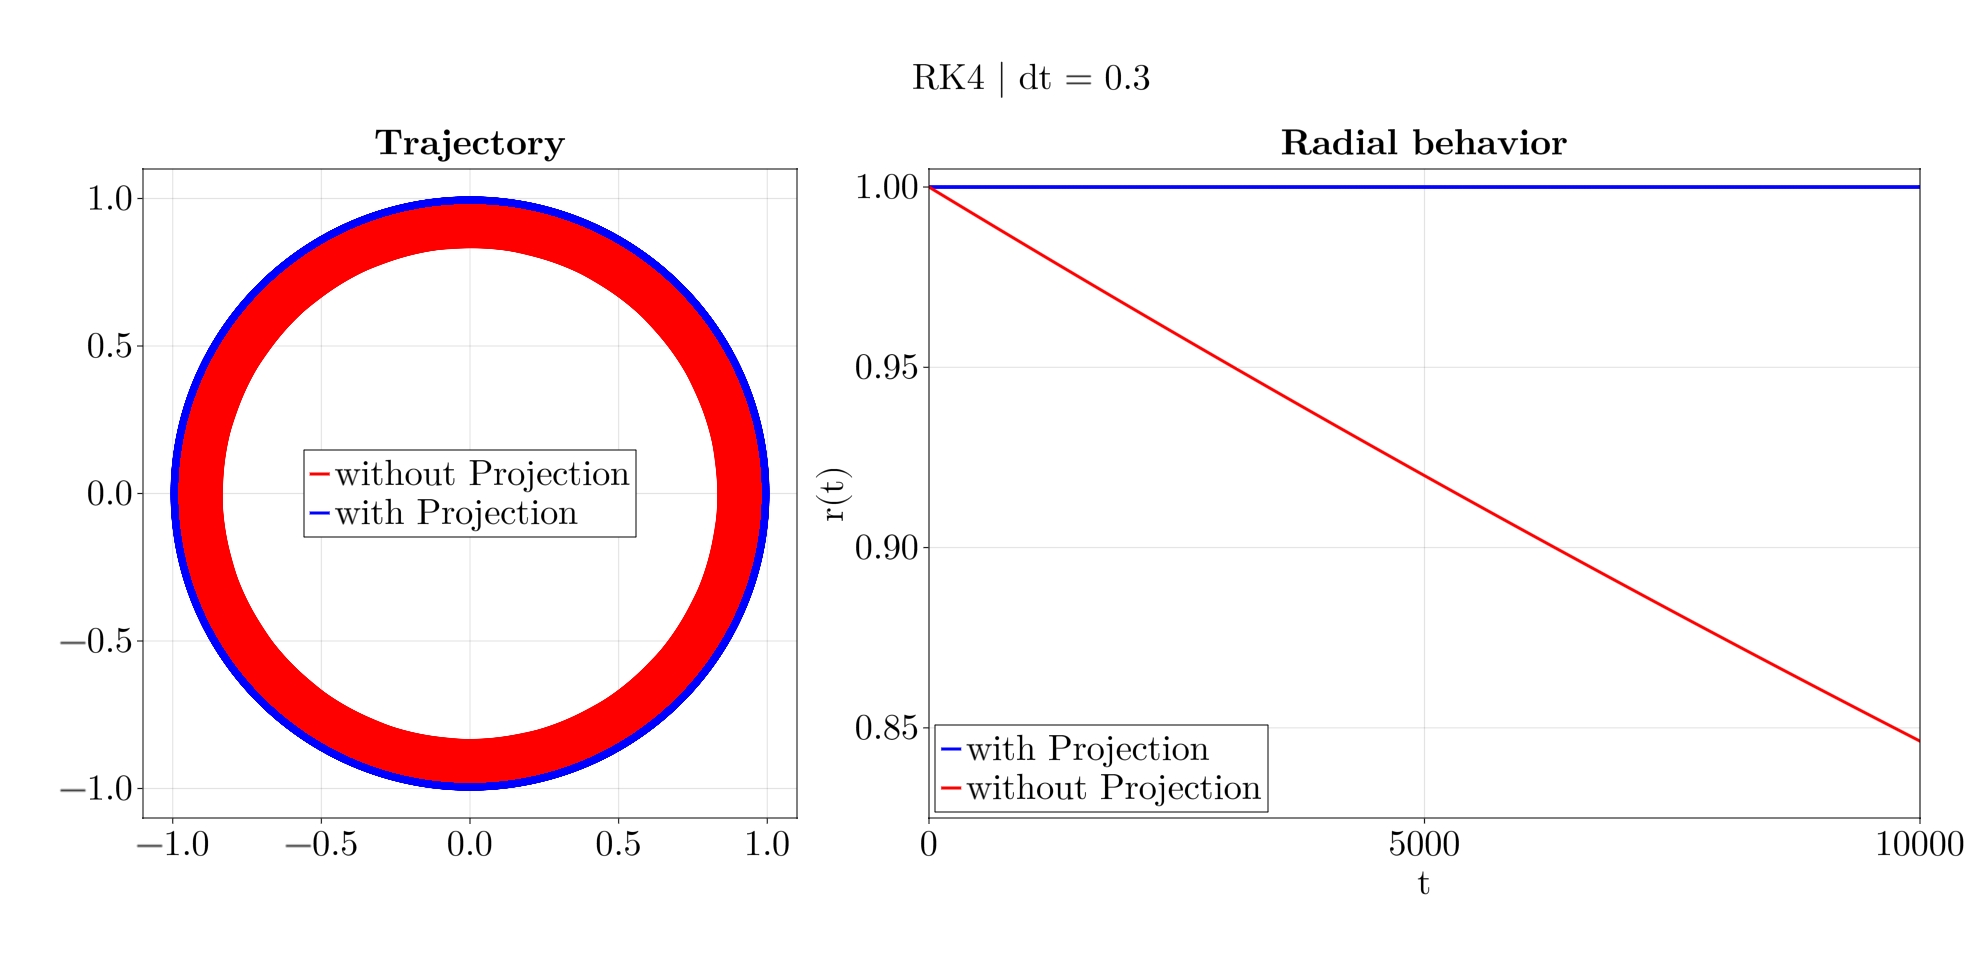
\includegraphics[width=0.8\textwidth, height=0.4\textwidth]{figures/manifold_projection_static.png}
				}
			}
		\end{center}
	\end{frame}
	
	\section{Validation}
	
	\begin{frame}{Validation Strategy}
		\begin{itemize}
			\item Test on three fundamental orbit classes in near-extremal Kerr ($a=0.998$):
			\begin{enumerate}
				\item \textbf{Scattering:} $|b| > b_c$ - photon escapes
				\item \textbf{Spiral:} $|b| \approx b_c$ - multiple windings (chaotic)
				\item \textbf{Capture:} $|b| < b_c$ - falls into horizon
			\end{enumerate}
			\item Monitor: $\Delta E/E_0$, $\Delta L_z/L_{z0}$, and null constraint violation.
		\end{itemize}
	\end{frame}
	
	\begin{frame}{Scattering Orbit}
		\begin{itemize}
			\item Photon approaches, reaches $r_{\min}$, escapes (``V'' shape in $r(\lambda)$).
		\end{itemize}
		\begin{figure}
			\centering
			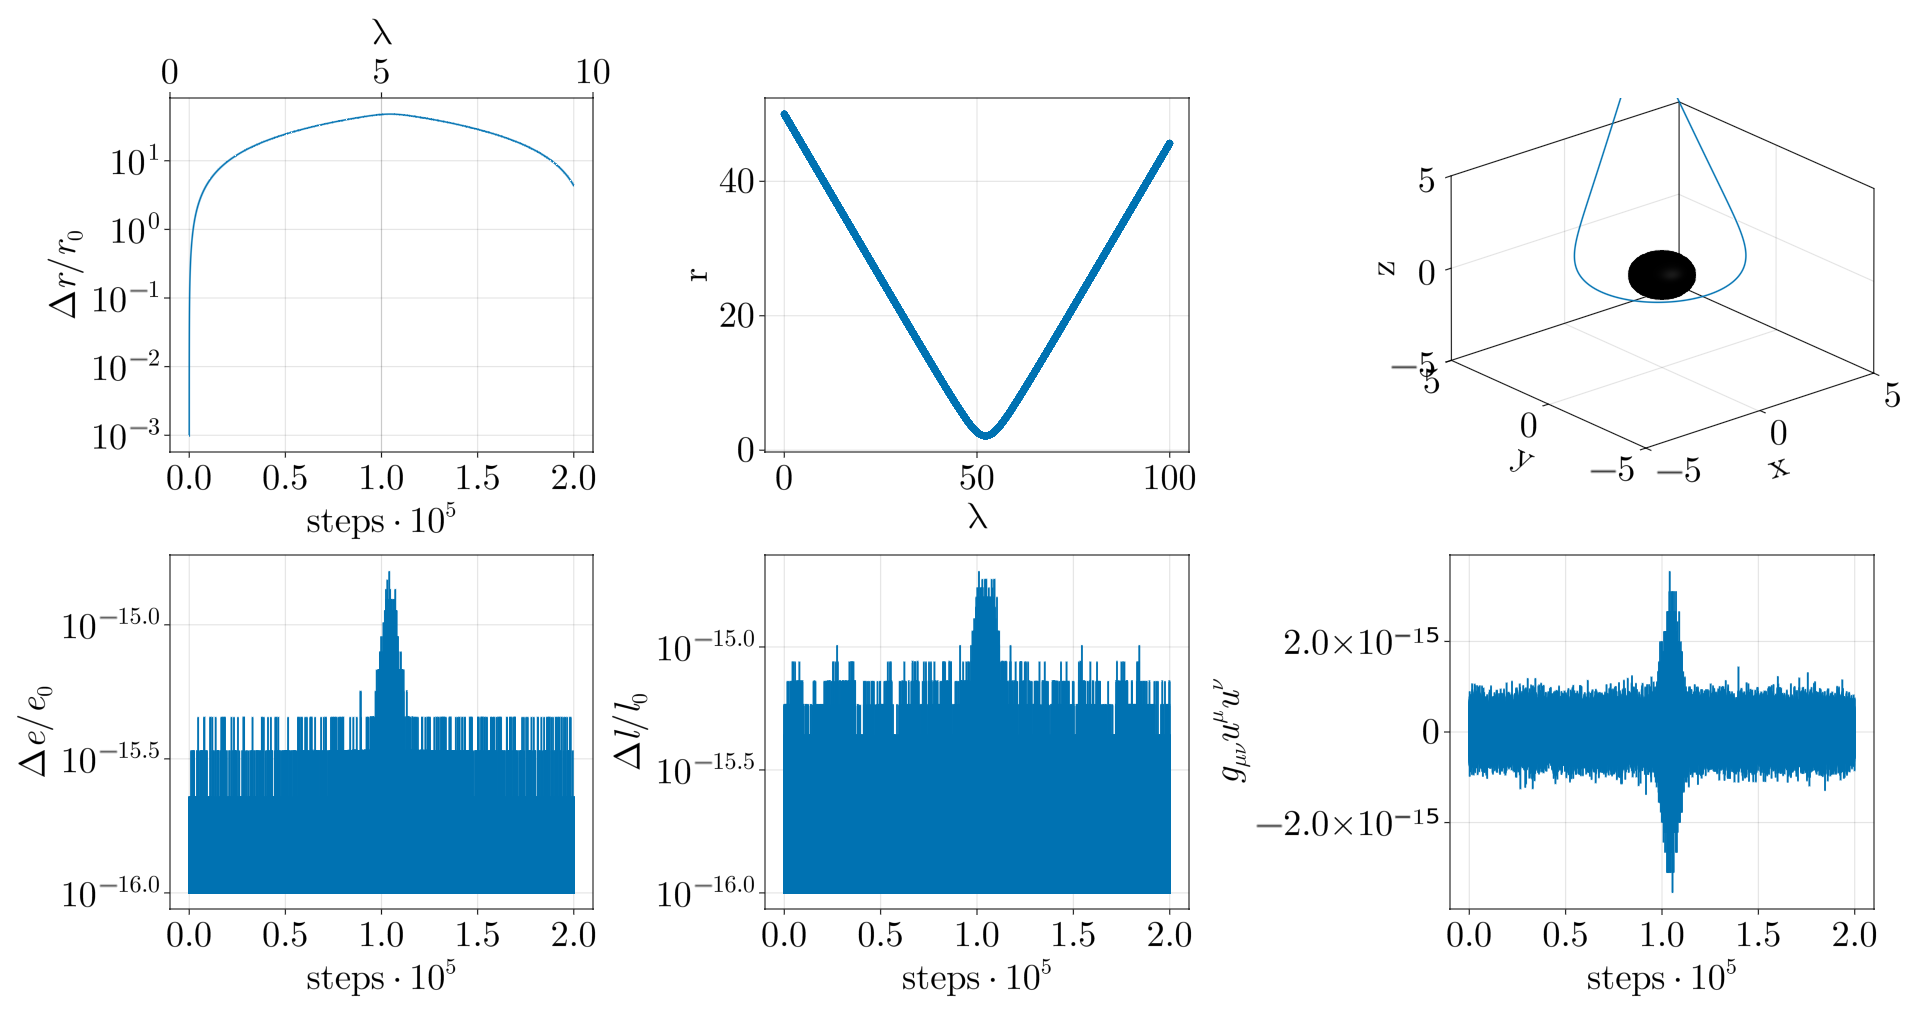
\includegraphics[width=0.8\textwidth]{figures/errors_V.png}
		\end{figure}
	\end{frame}
	
	\begin{frame}{The Stress Test: Unstable Spiral}
		\begin{itemize}
			\item Photon orbits near the photon sphere - extreme Lyapunov sensitivity.
		\end{itemize}
		\begin{figure}
			\centering
			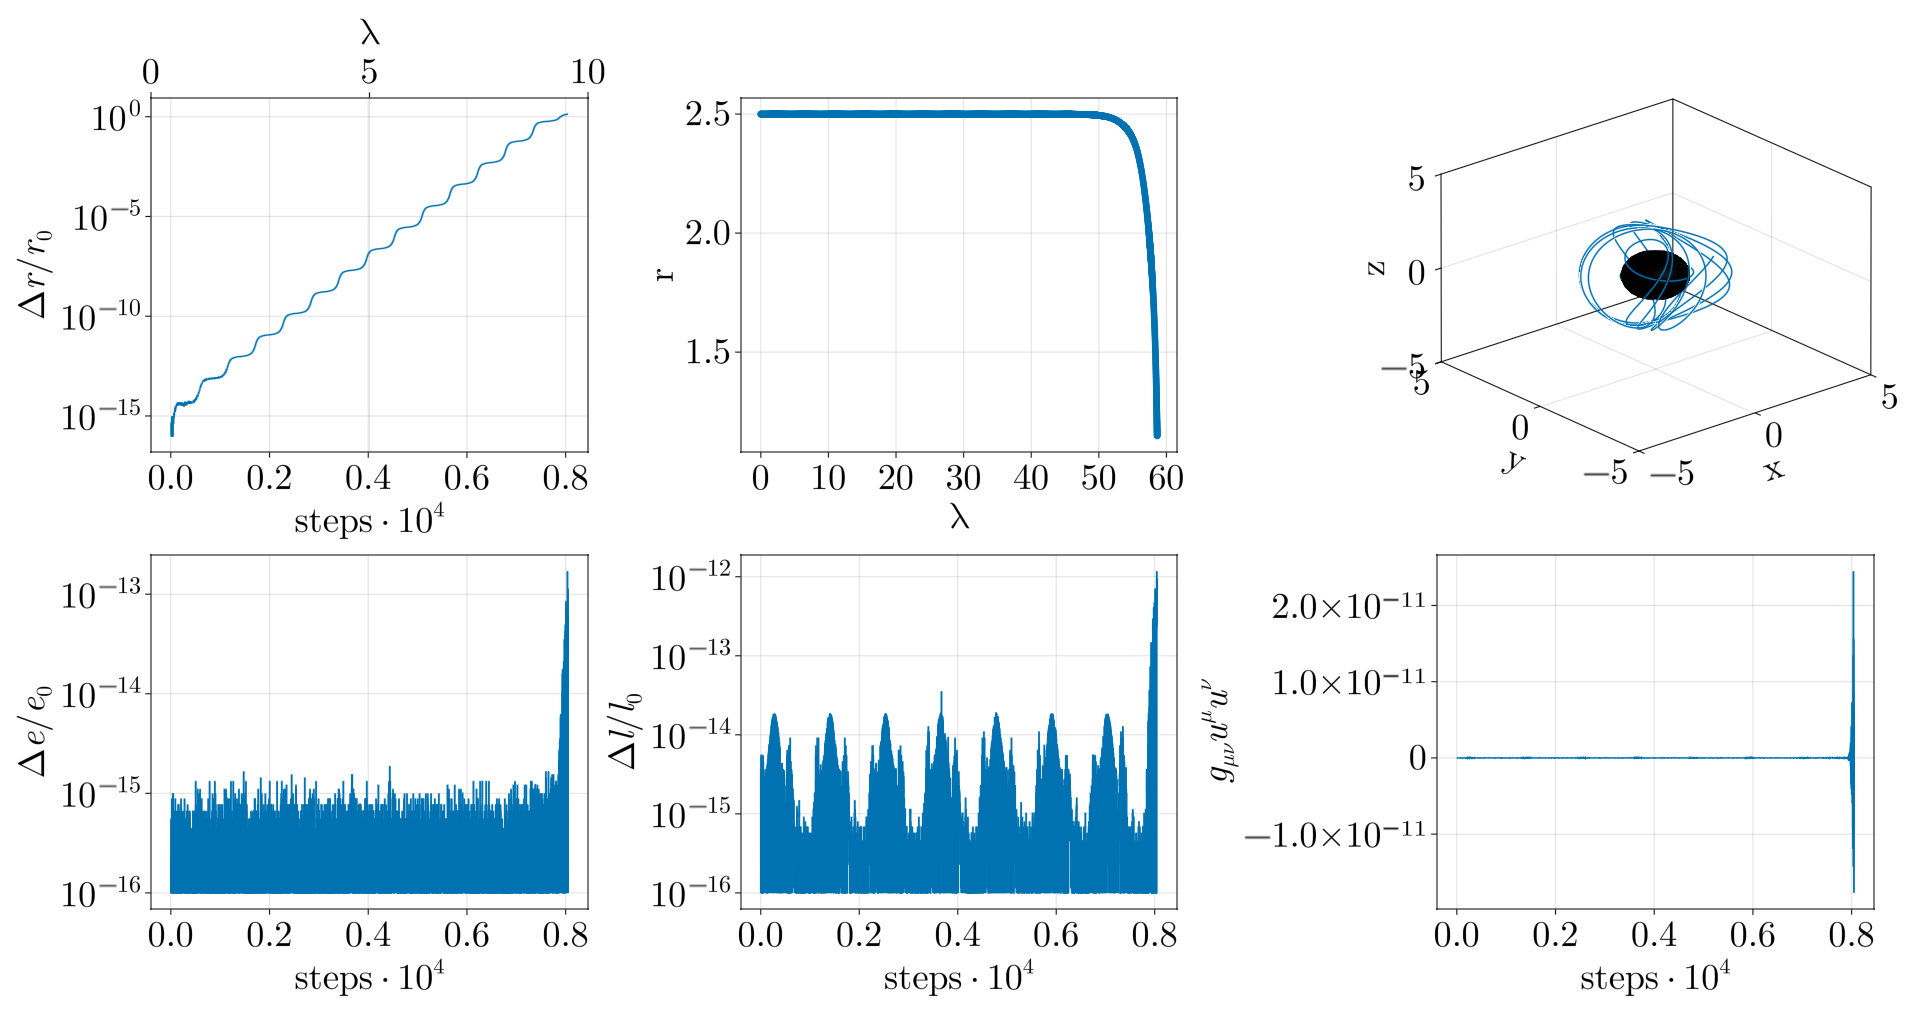
\includegraphics[width=0.8\textwidth]{figures/errors_stable.png}
		\end{figure}
	\end{frame}
	
	\begin{frame}{Direct Capture}
		\begin{itemize}
			\item Photon plunges monotonically into the horizon.
		\end{itemize}
		\begin{figure}
			\centering
			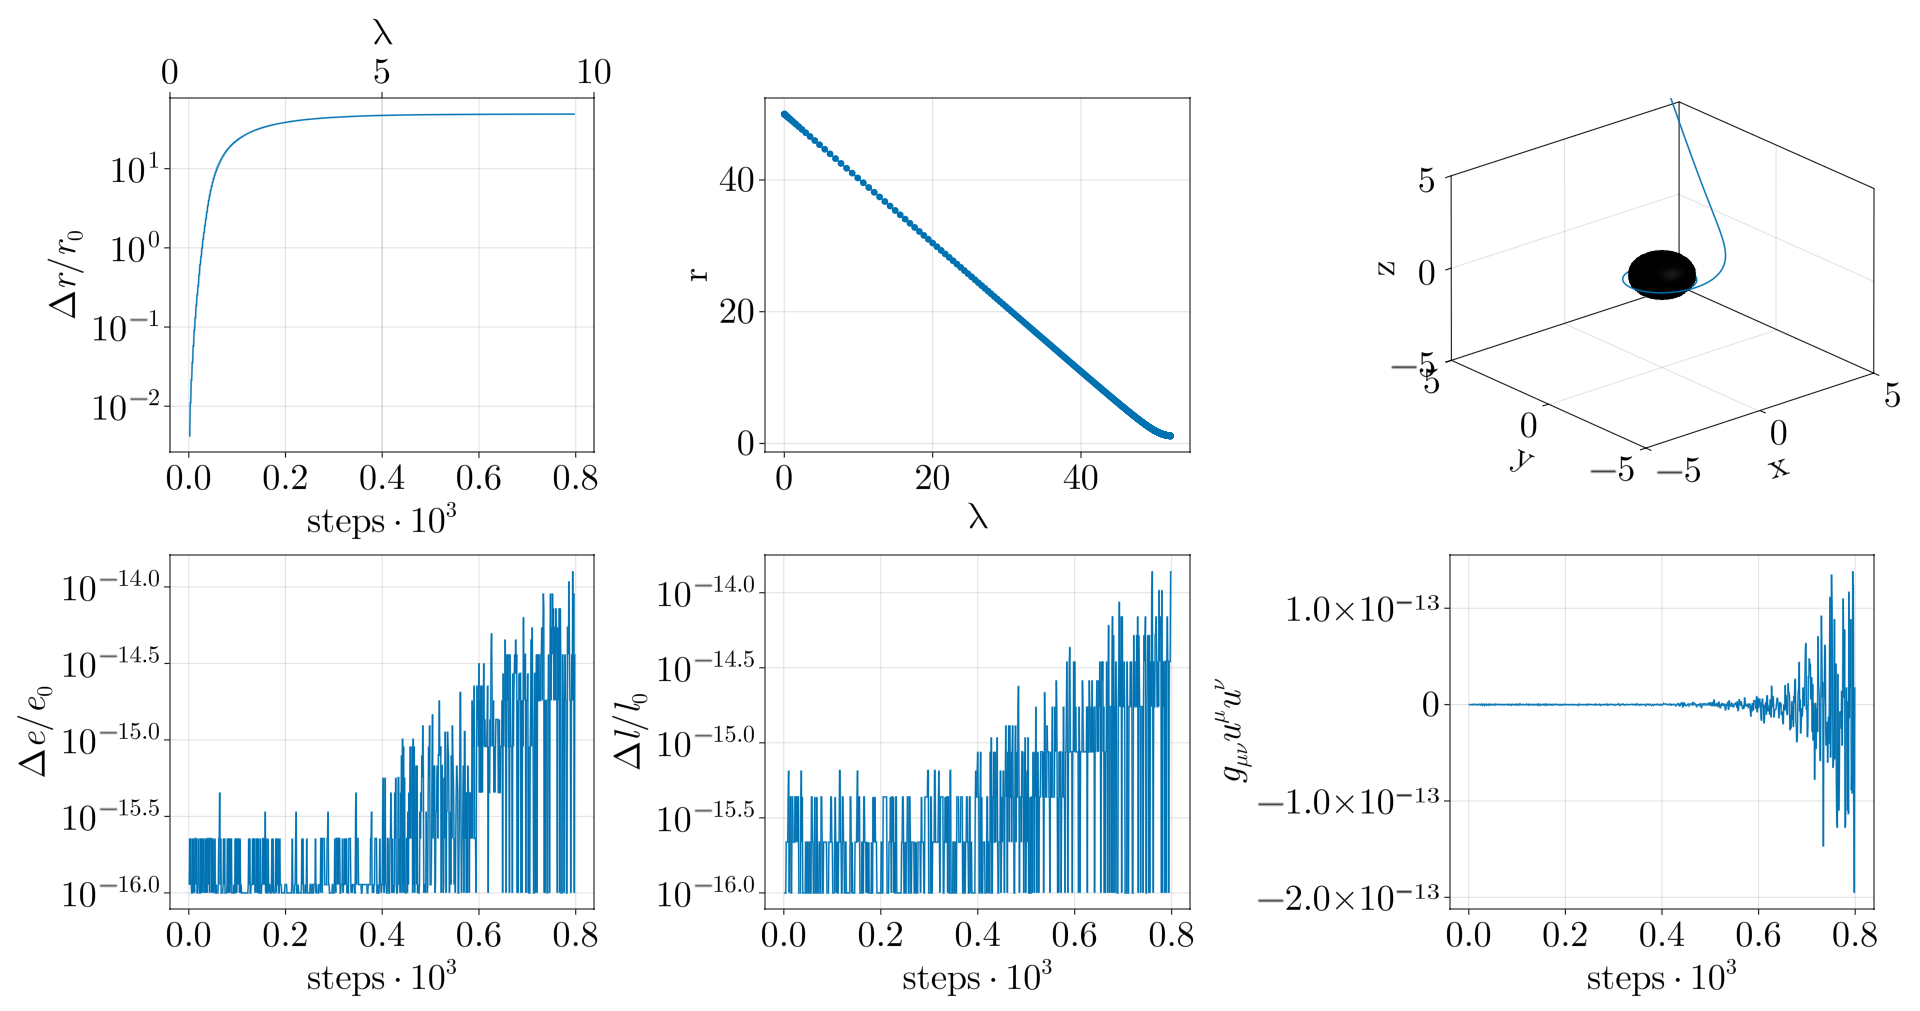
\includegraphics[width=0.8\textwidth]{figures/errors_cap.png}
		\end{figure}
	\end{frame}
	
	\section{Imaging Methodology}
	
	\begin{frame}{How We Compute the Shadow}
		\begin{itemize}
			\item \textbf{Backward Ray Tracing:} We place a virtual camera at distance $r_0 \gg M$ and inclination $\theta_0$.
			\item \textbf{For each pixel:} Trace the photon backwards in time.
			\begin{itemize}
				\item If it crosses the horizon $\rightarrow$ black pixel (shadow).
				\item If it escapes $\rightarrow$ map to background image.
			\end{itemize}
		\end{itemize}
		\vspace{0.3cm}
		\begin{block}{The Shadow Boundary}
			The shadow edge corresponds to photons that asymptotically approach the unstable photon sphere - the most numerically demanding trajectories.
		\end{block}
	\end{frame}
	
	\begin{frame}{Calibration: The 4-Color Test Image}
		\begin{itemize}
			\item \textbf{Why calibrate?} Before using realistic backgrounds, we must verify the \textbf{UV mapping} and \textbf{handedness} of the celestial sphere projection.
			\item \textbf{The test:} A simple equirectangular image with 4 distinct quadrants (red, green, blue, yellow).
			\item \textbf{What we check:} After gravitational lensing, the colors must appear in the physically correct positions - confirming that our coordinate conventions match the spacetime geometry.
		\end{itemize}
		\begin{center}
			
\includegraphics[width=0.32\textwidth]{figures/test_image.jpg}
		\end{center}
	\end{frame}
	
	\begin{frame}{Educational Animation: Ray Tracing in Action}
		\begin{itemize}
			\item We ``shoot'' one virtual photon from each pixel of the observer's screen backwards in time.
			\item These rays travel through the curved spacetime of the black hole, following exact geodesic equations.
			\item The final destination of each ray (e.g., hitting the accretion disk, falling into the event horizon, or escaping to background stars) dictates the exact color assigned to that pixel.
		\end{itemize}
		\begin{center}
			\href{run:figures/edu2.mp4}{
				\fbox{
					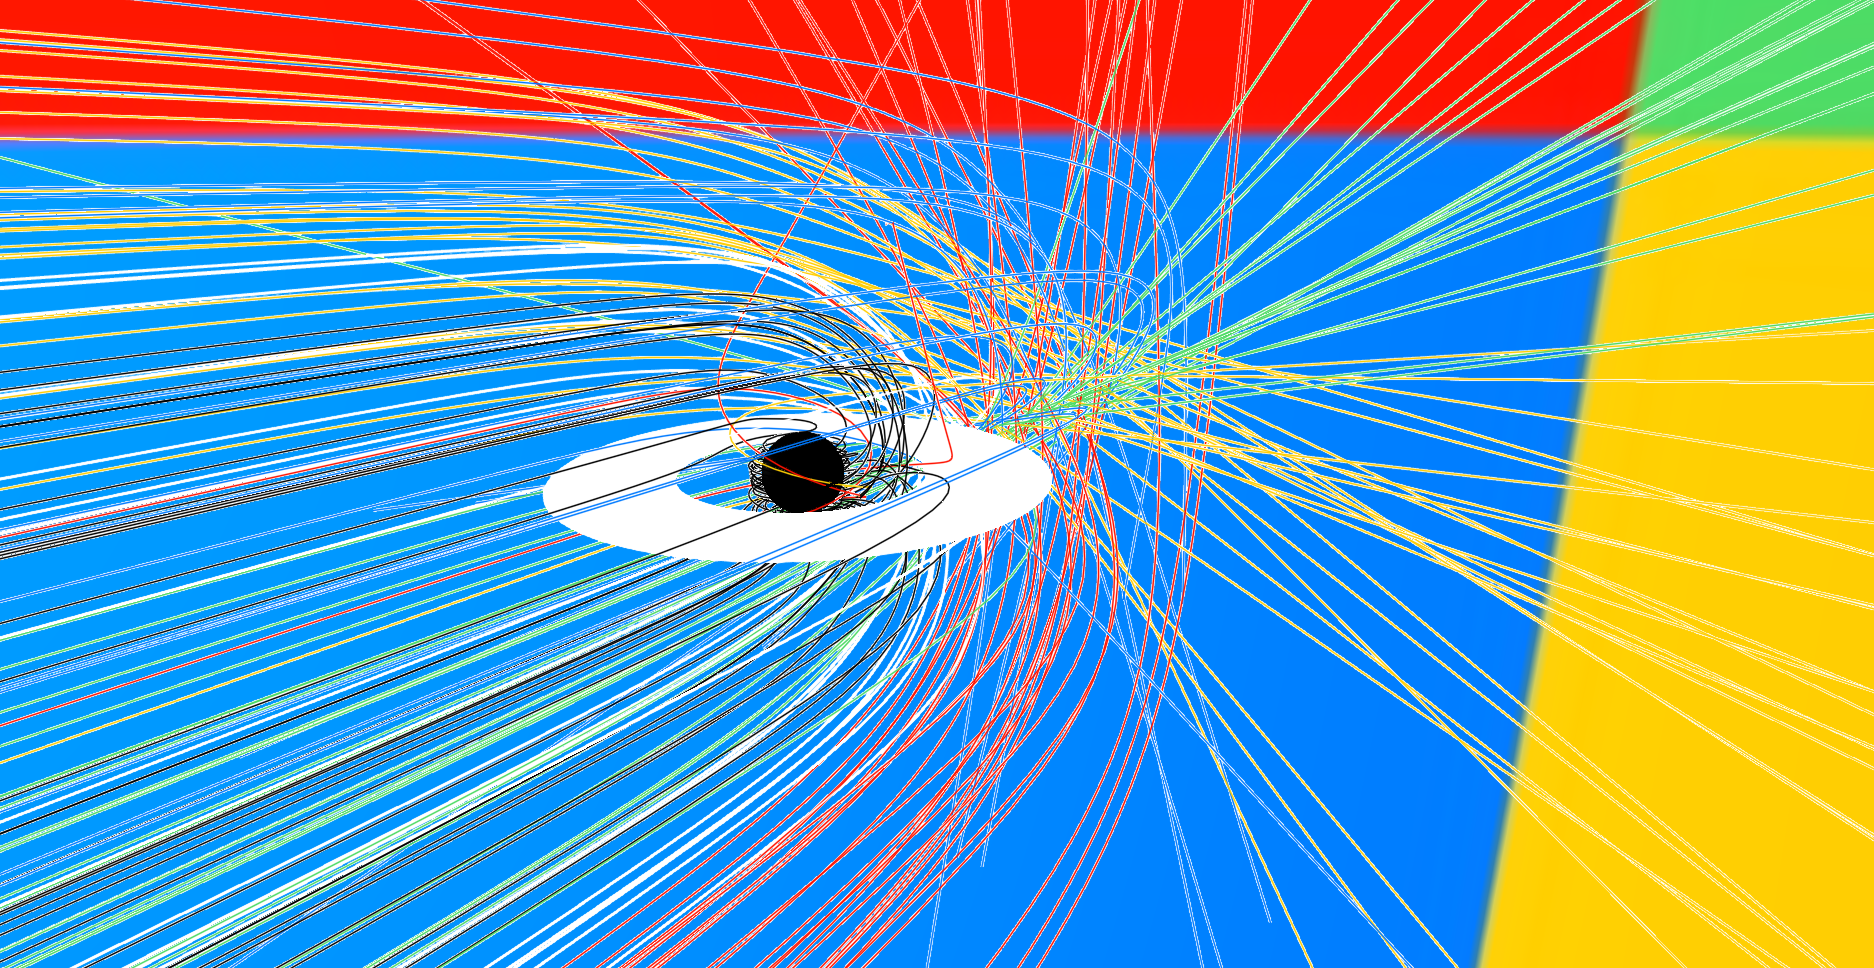
\includegraphics[width=0.6\textwidth, height=0.3\textwidth]{figures/edu.png}
				}
			}
		\end{center}
	\end{frame}
	
	\begin{frame}{Calibration: Lensed Result}
		\begin{center}
			The same 4-color image, now lensed by a near-extremal Kerr black hole ($a=0.998$).
		\end{center}
		\begin{columns}
			\begin{column}{0.45\textwidth}
				\textbf{Observations:}
				\begin{itemize}
					\item The central black region is the \textbf{shadow} (photons captured by the horizon).
					\item The white ring is the \textbf{photon ring} (photons that orbited the black hole).
					\item The colors are distorted and wrapped around the shadow, confirming correct handedness.
					\item The ``D'' shape asymmetry is clearly visible due to frame-dragging.
				\end{itemize}
			\end{column}
			\begin{column}{0.4\textwidth}
				\centering
				
\includegraphics[width=\textwidth]{figures/trace_rad_2000x2000_test.png}
			\end{column}
		\end{columns}
	\end{frame}
	
	\section{Results: Imaging}
	
	\begin{frame}{Gravitational Lensing: Point Source Test}
		\begin{itemize}
			\item \textbf{Setup:} A single point source (red dot) placed directly behind the black hole.
			\item \textbf{What we observe:}
			\begin{itemize}
				\item \textbf{Primary \& Secondary Arcs:} Photons passing on either side of the black hole ($n=0, 1$).
				\item \textbf{Higher-order Sub-rings:} Photons that orbited multiple times ($n \geq 2$), visible as tiny dots near the shadow boundary.
			\end{itemize}
		\end{itemize}

		\begin{columns}
			\begin{column}{0.3\textwidth}
				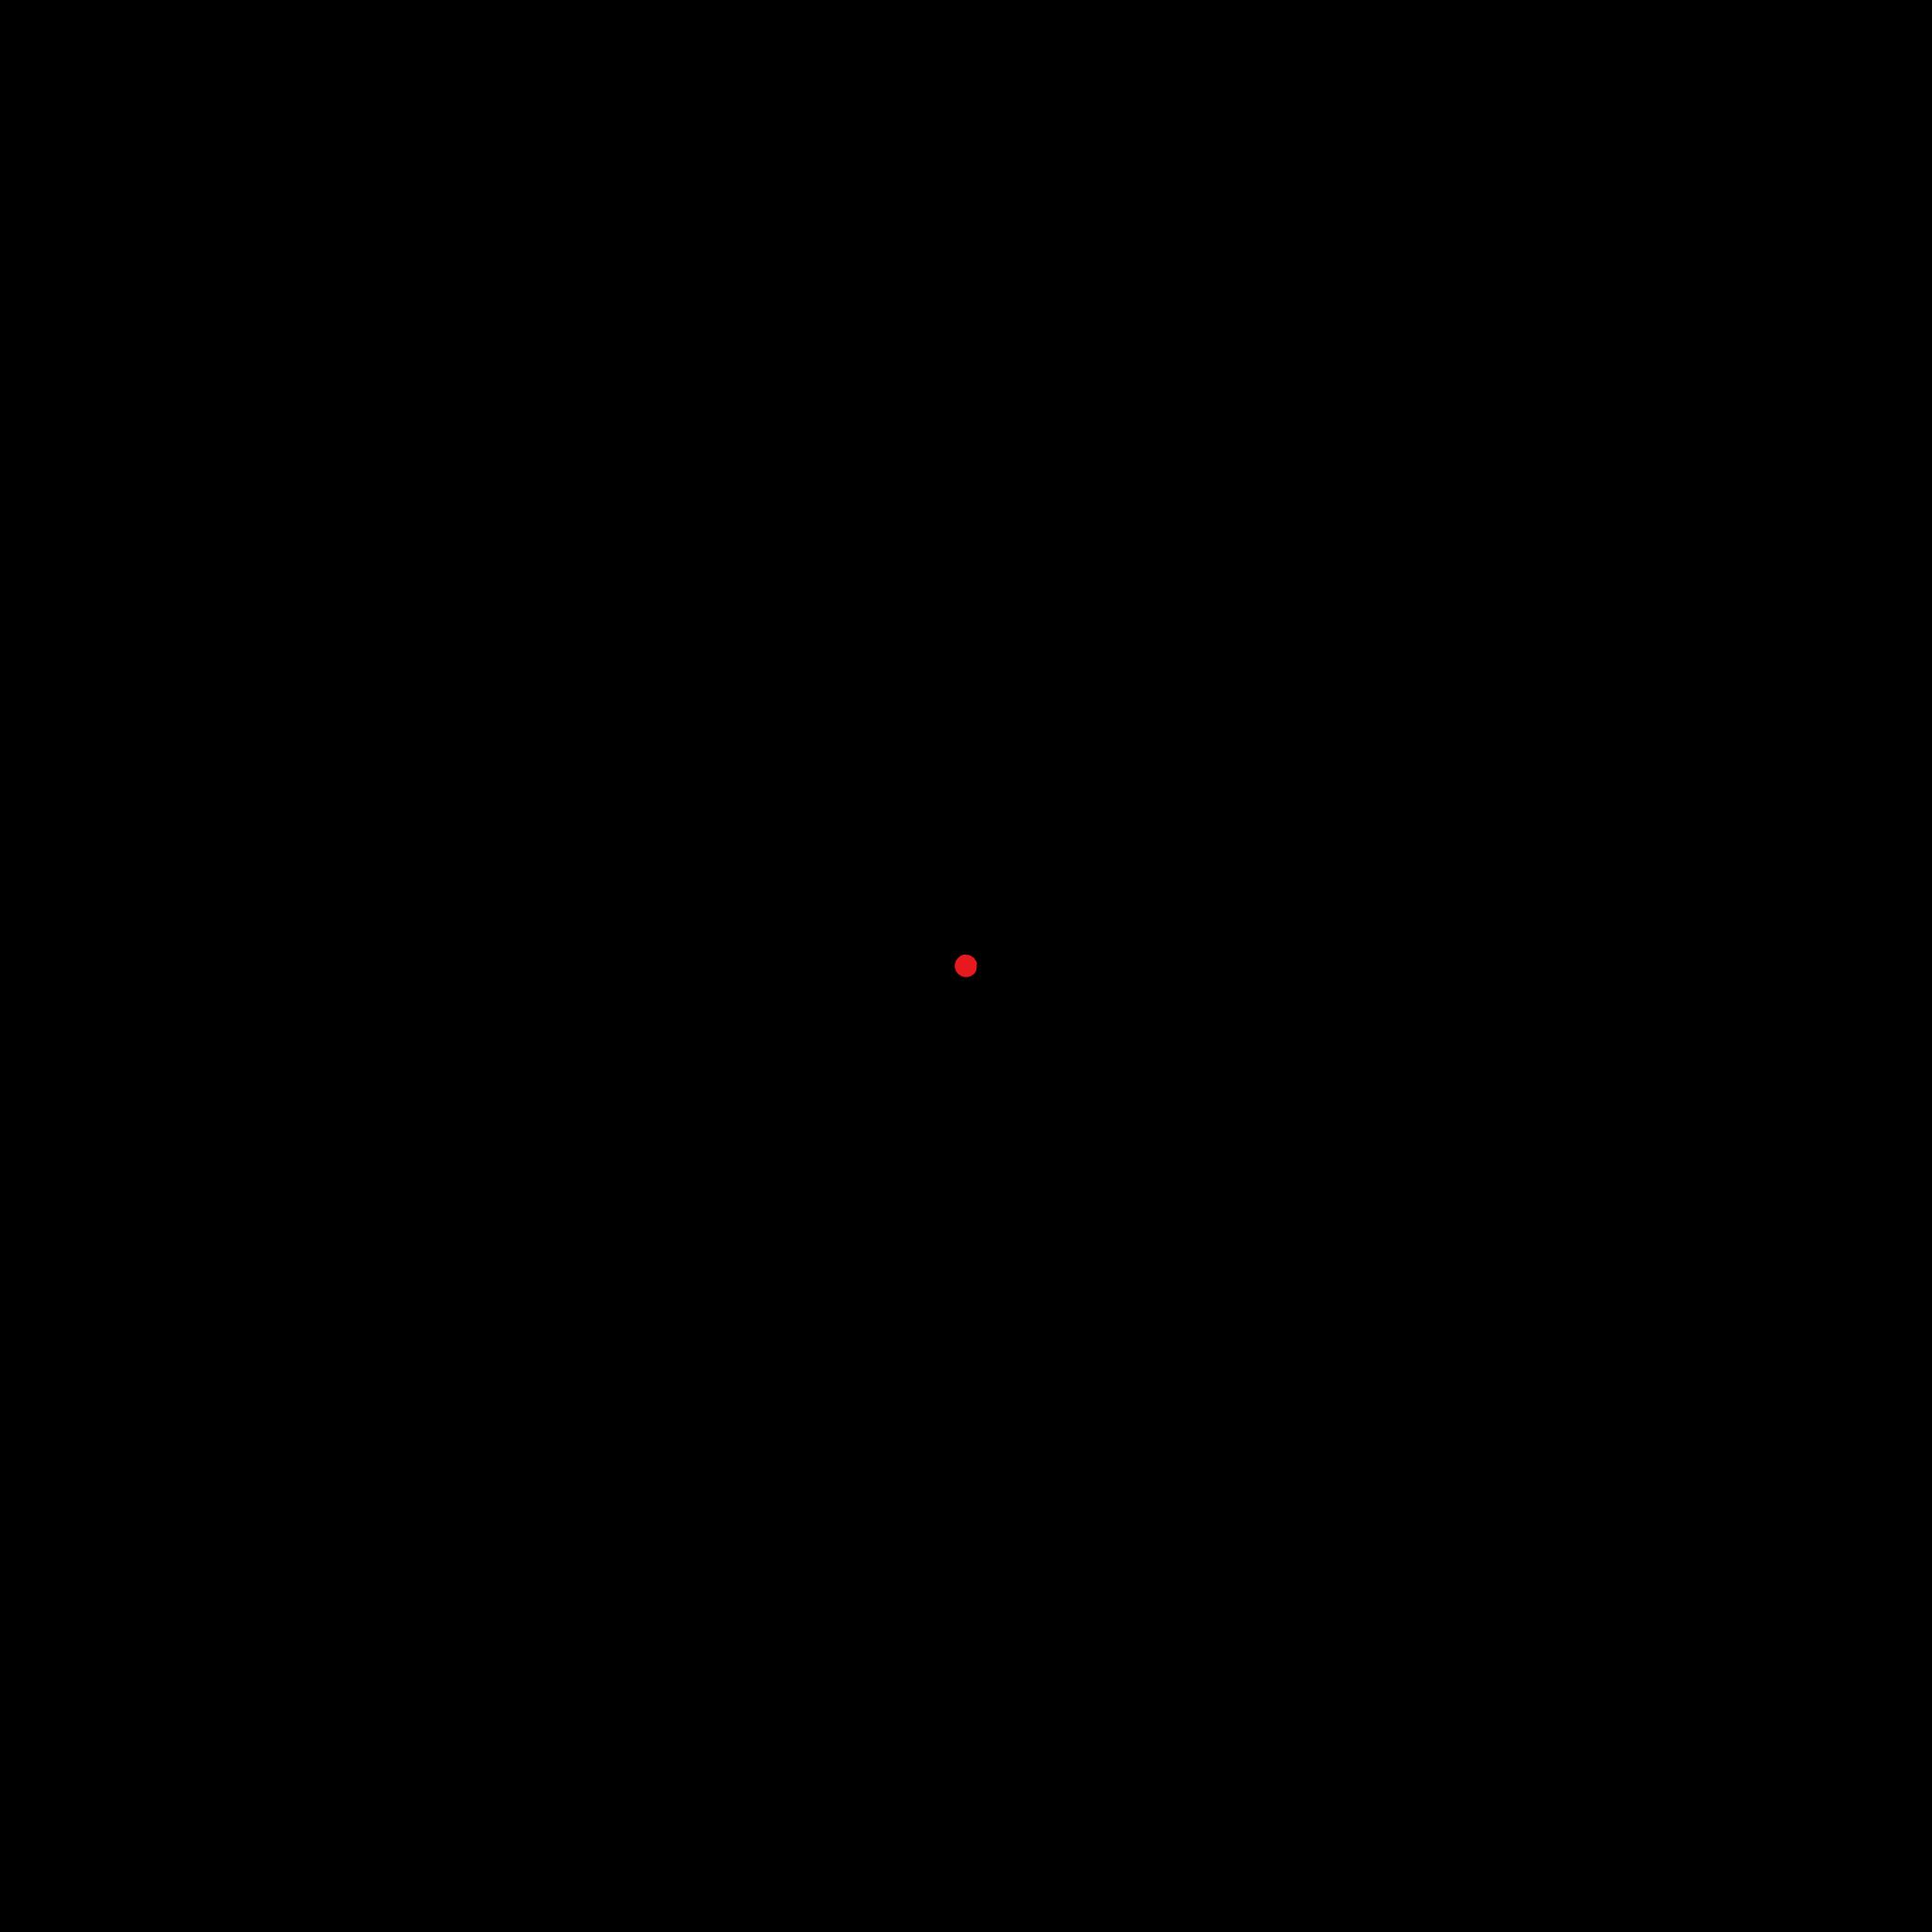
\includegraphics[width=\textwidth]{figures/dot.jpg}
			\end{column}
			\begin{column}{0.35\textwidth}
				
\includegraphics[width=\textwidth]{figures/trace_rad_1000x1000_dot_shadow.png}
			\end{column}
		\end{columns}
	\end{frame}
	
	\begin{frame}{Realistic Imaging: Milky Way Background - Source}
		\begin{itemize}
			\item Escaping rays are mapped to an equirectangular Milky Way image.
			\item Calibration with the 4-color test image ensures correct handedness and physical orientation.
		\end{itemize}
		\begin{figure}
			\centering
			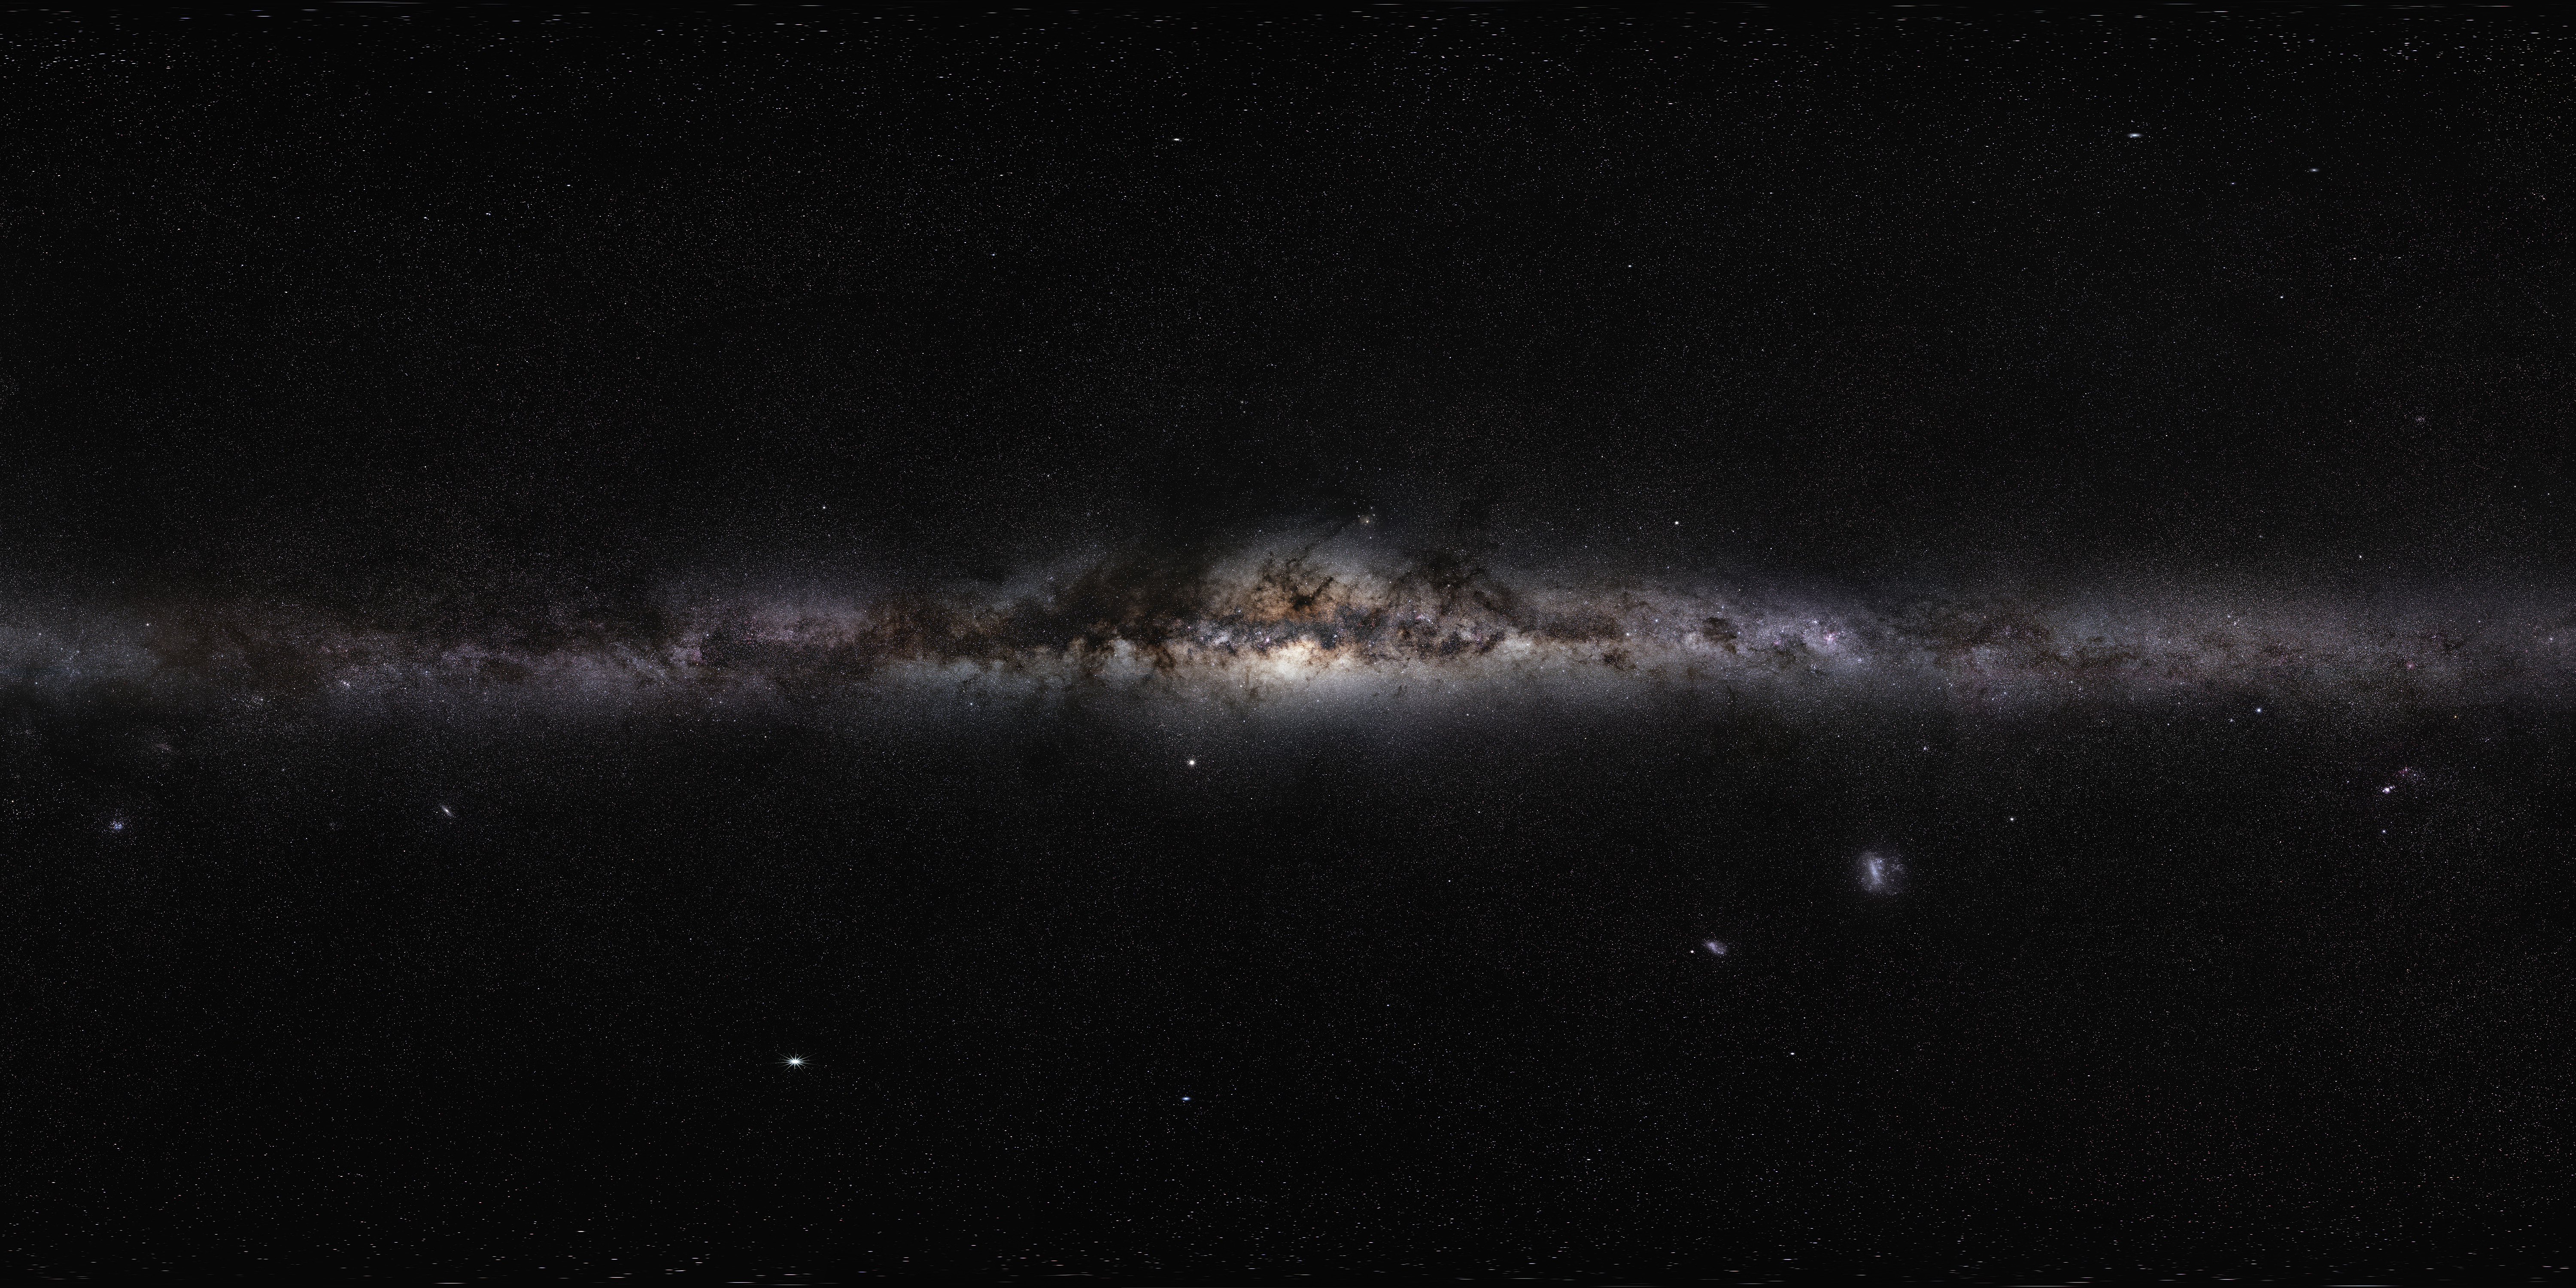
\includegraphics[width=0.7\textwidth]{figures/milky_way.jpg}
		\end{figure}
	\end{frame}
	
	\begin{frame}{Realistic Imaging: Milky Way Background - Result}
		\centering This demonstrates pure gravitational lensing of a realistic background, without local emission.
		\begin{figure}
			\centering
			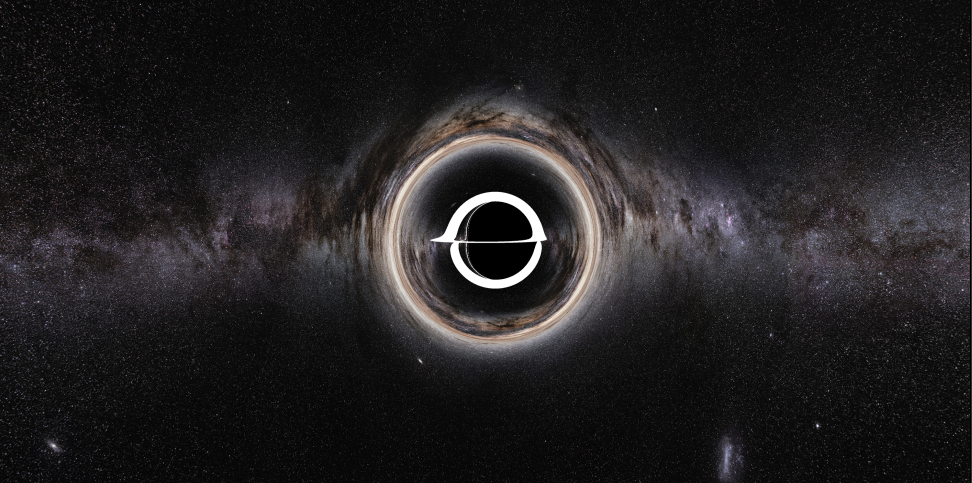
\includegraphics[width=0.9\textwidth]{figures/milkyway_tracing.png}
		\end{figure}
	\end{frame}
	
	\begin{frame}{Frame Dragging Evolution}
		\begin{center}
		As spin $a$ increases, the spacetime geometry is dragged along the rotation direction.
		\end{center}
	\vspace{0.5 cm}
		\begin{columns}
			\column{0.5\textwidth}
			\centering
			\textbf{Schwarzschild ($a=0$)} \\
			\href{run:figures/frame_dragging_animation_a0.0.mp4}{
				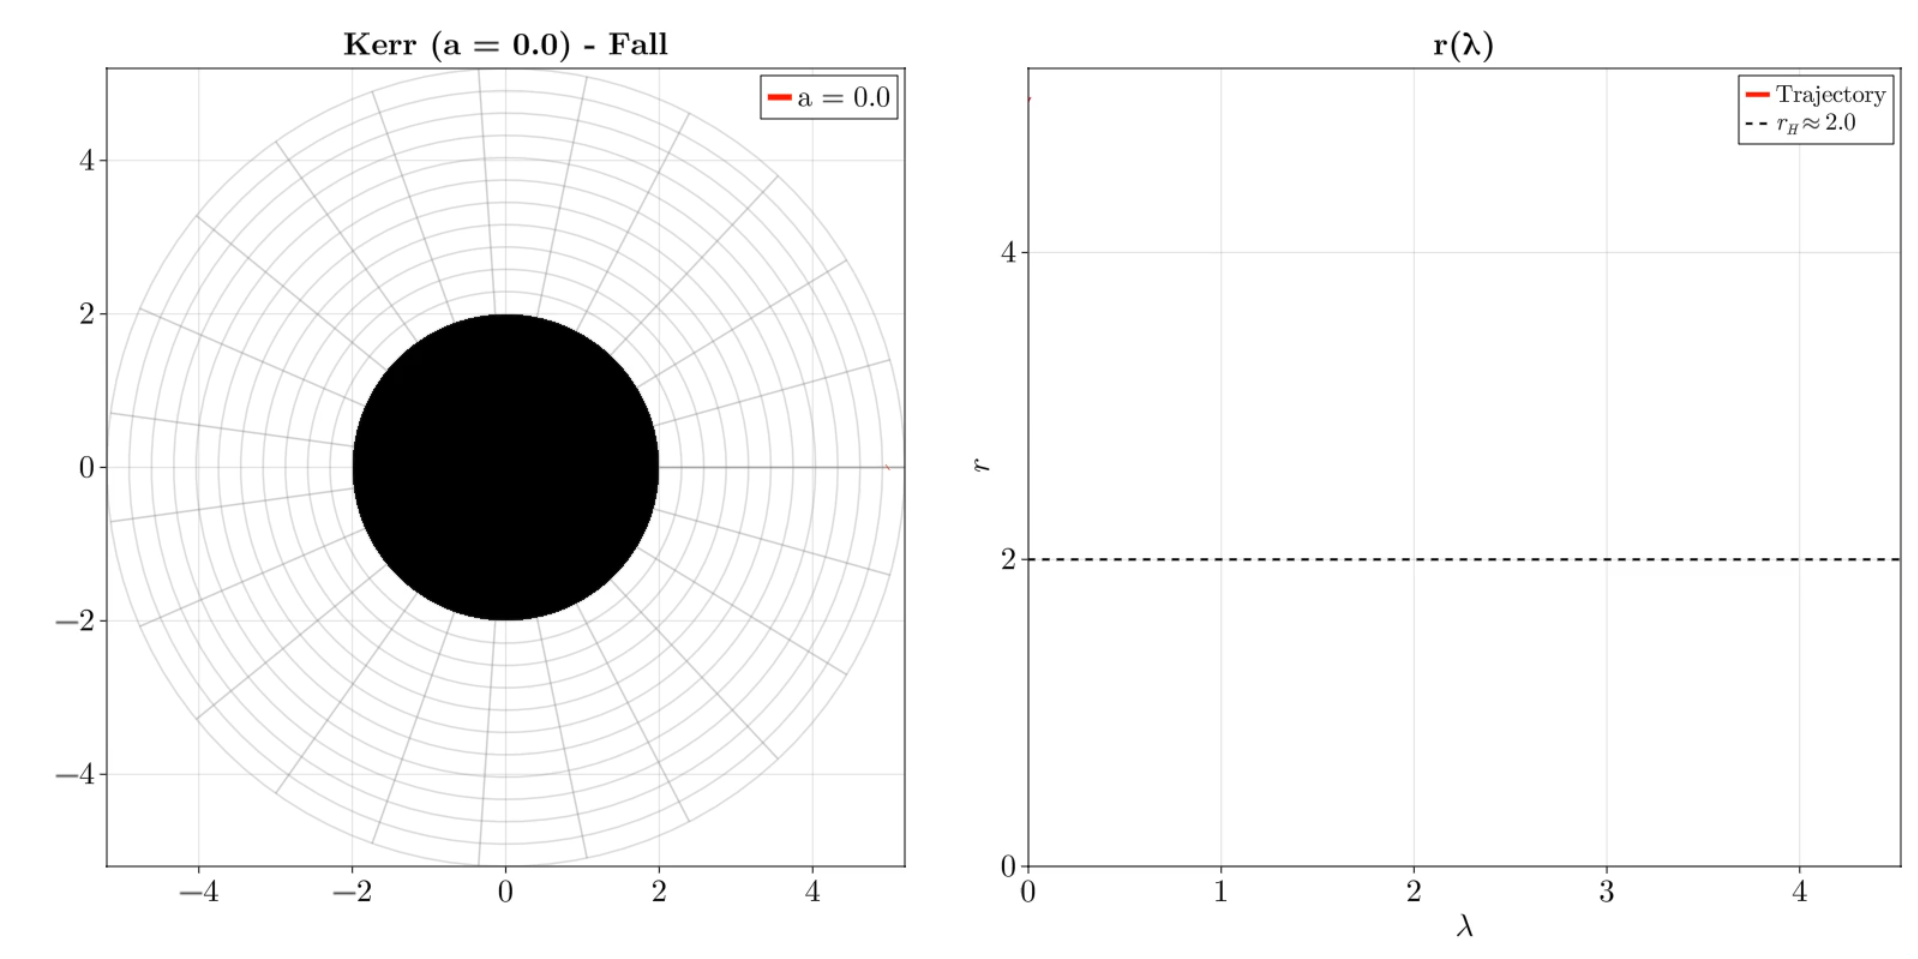
\includegraphics[width=0.85\textwidth]{figures/fd_a0.png}
			}
			
			\column{0.5\textwidth}
			\centering
			\textbf{Near-Extremal Kerr ($a=0.998$)} \\
			\href{run:figures/frame_dragging_animation_a0.998.mp4}{
				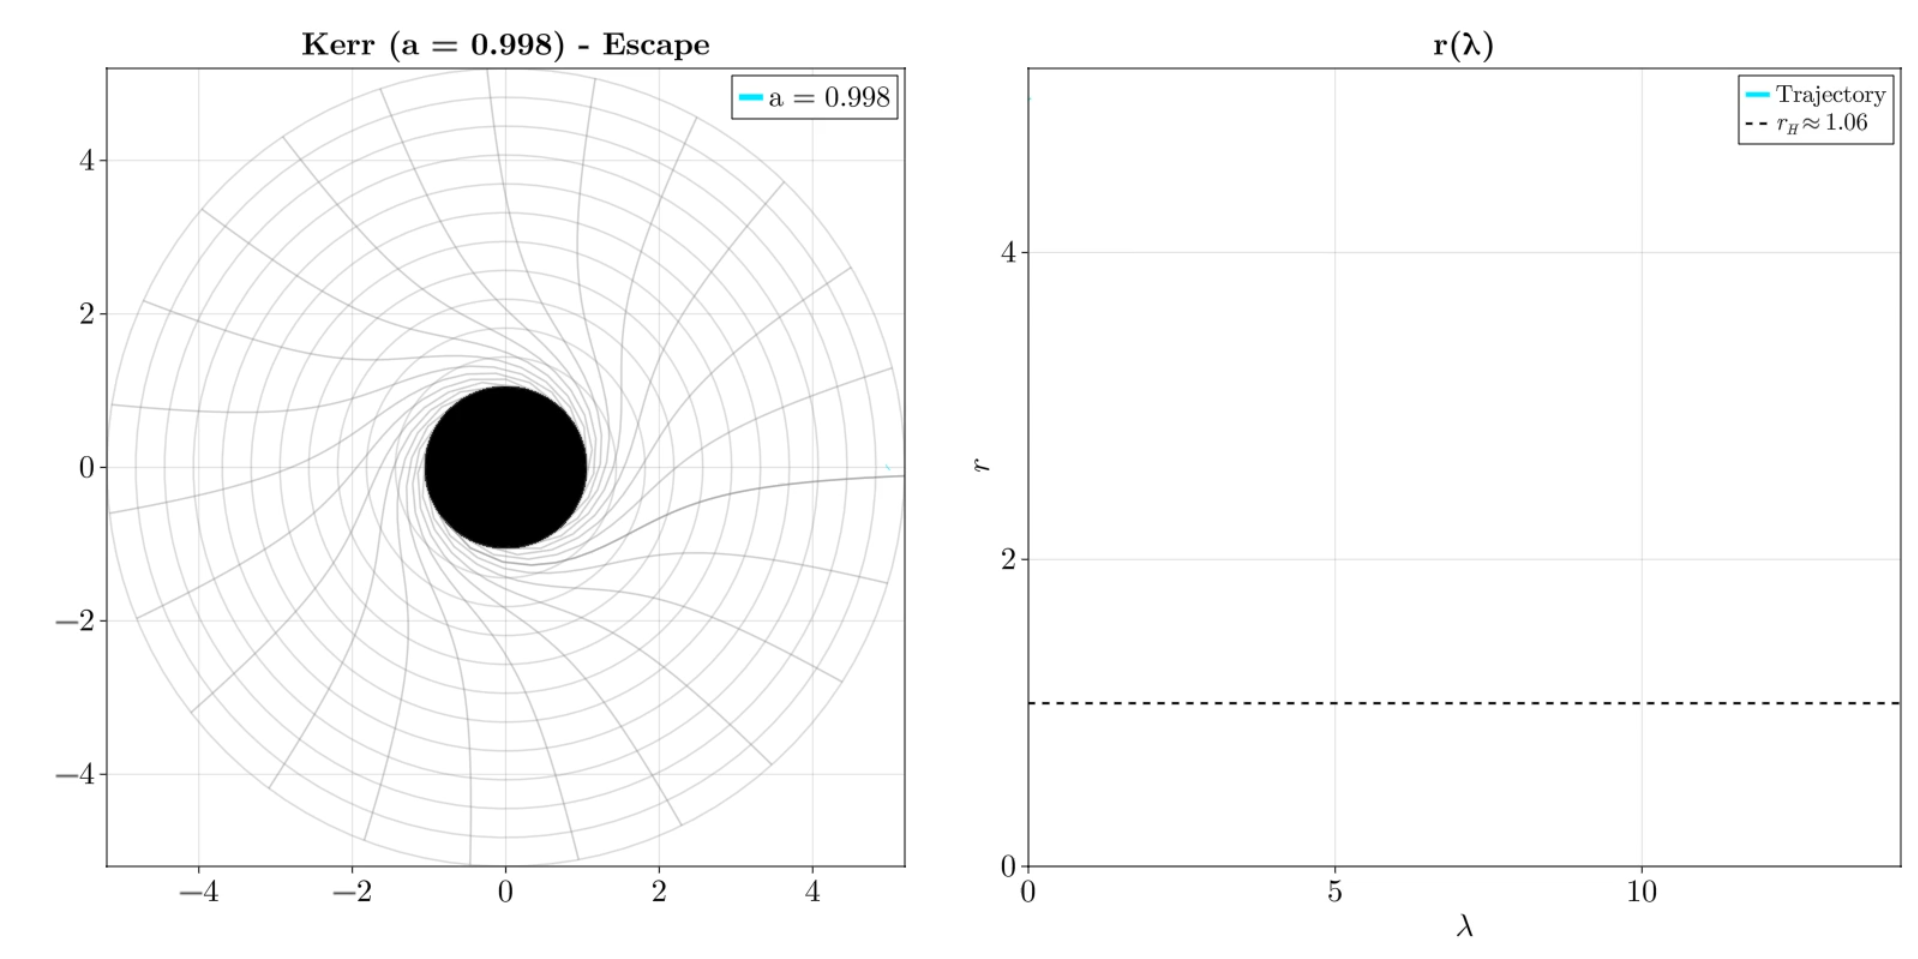
\includegraphics[width=0.85\textwidth]{figures/fd_a0998.png}
			}
		\end{columns}
	\end{frame}

	\begin{frame}{Plasma Model: Thin Accretion Disk}
		\begin{itemize}
			\item \textbf{Physical setup:} Geometrically thin, optically thick accretion disk in the equatorial plane ($\theta = \pi/2$).
			\item \textbf{Emission profile:} Local emissivity $\epsilon(r)$ follows an exponential density profile, peaking near the Innermost Stable Circular Orbit (ISCO) for each spin parameter..
			\item \textbf{Radiative transfer:} The observed intensity along each ray is:
			\begin{equation}
				I_{\text{obs}} = \int g^4 \, \epsilon(r) \, d\lambda
			\end{equation}
			where $g$ is the relativistic redshift factor.
		\end{itemize}
		\vspace{0.3cm}
		\begin{block}{Key Relativistic Effects}
			\begin{itemize}
				\item \textbf{Doppler beaming ($g^4$):} Approaching plasma appears much brighter than receding plasma.
				\item \textbf{Gravitational lensing:} Light from the far side of the disk is bent over and under the black hole.
				\item \textbf{Photon ring:} Multiple windings create a self-similar hierarchy of sub-rings near the shadow boundary.
			\end{itemize}
		\end{block}
	\end{frame}
	
	\begin{frame}{Shadow Morphology: Spin Dependence}
		\begin{itemize}
			\item The mathematical shadow is the region of captured photons.
			\item \textbf{Schwarzschild ($a=0$):} Perfectly circular shadow due to spherical symmetry.
			\item \textbf{Kerr ($a=0.998$):} Pronounced ``D'' shape asymmetry caused by frame-dragging.
		\end{itemize}
		\vspace{0.2cm}
		\begin{columns}
			\column{0.5\textwidth}
			\centering
			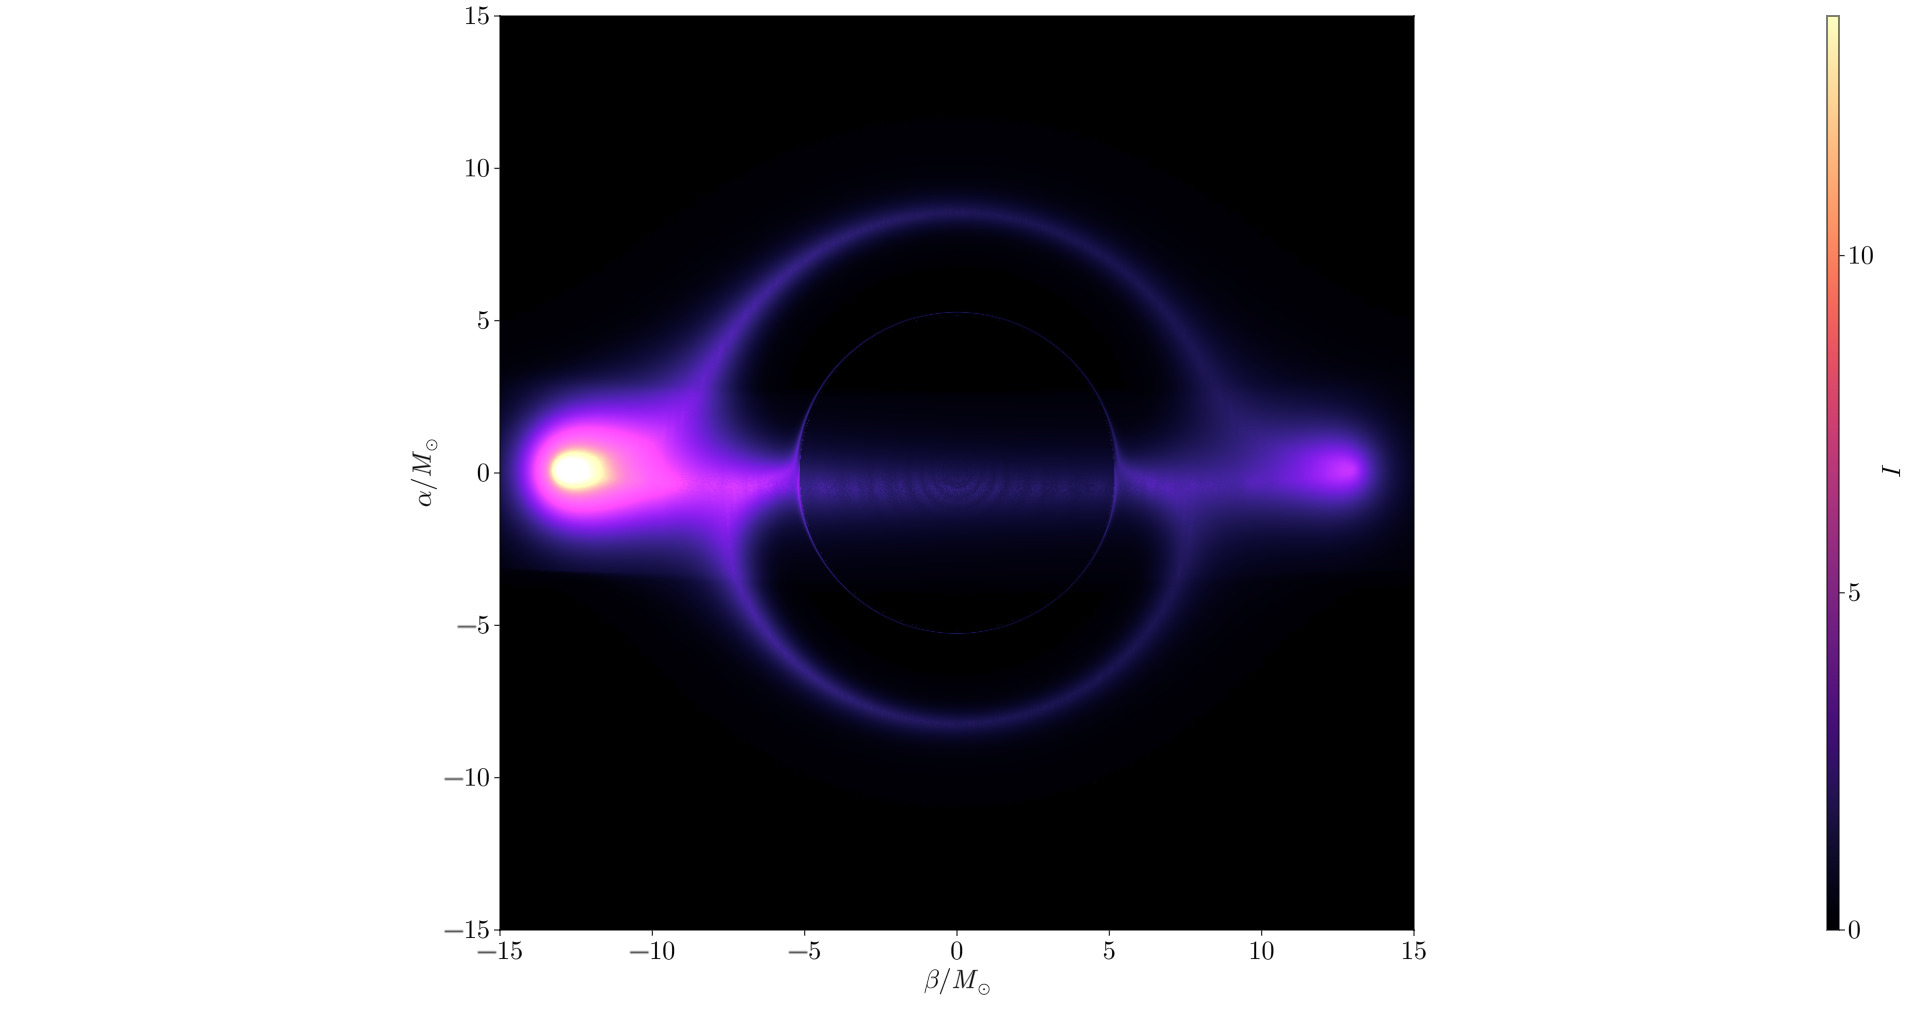
\includegraphics[width=1\textwidth]{figures/bh_shadow_1000x1000_a000.png}
			\captionof{Schwarzschild}{Perfect circle ($a=0$).}
			
			\column{0.5\textwidth}
			\centering
			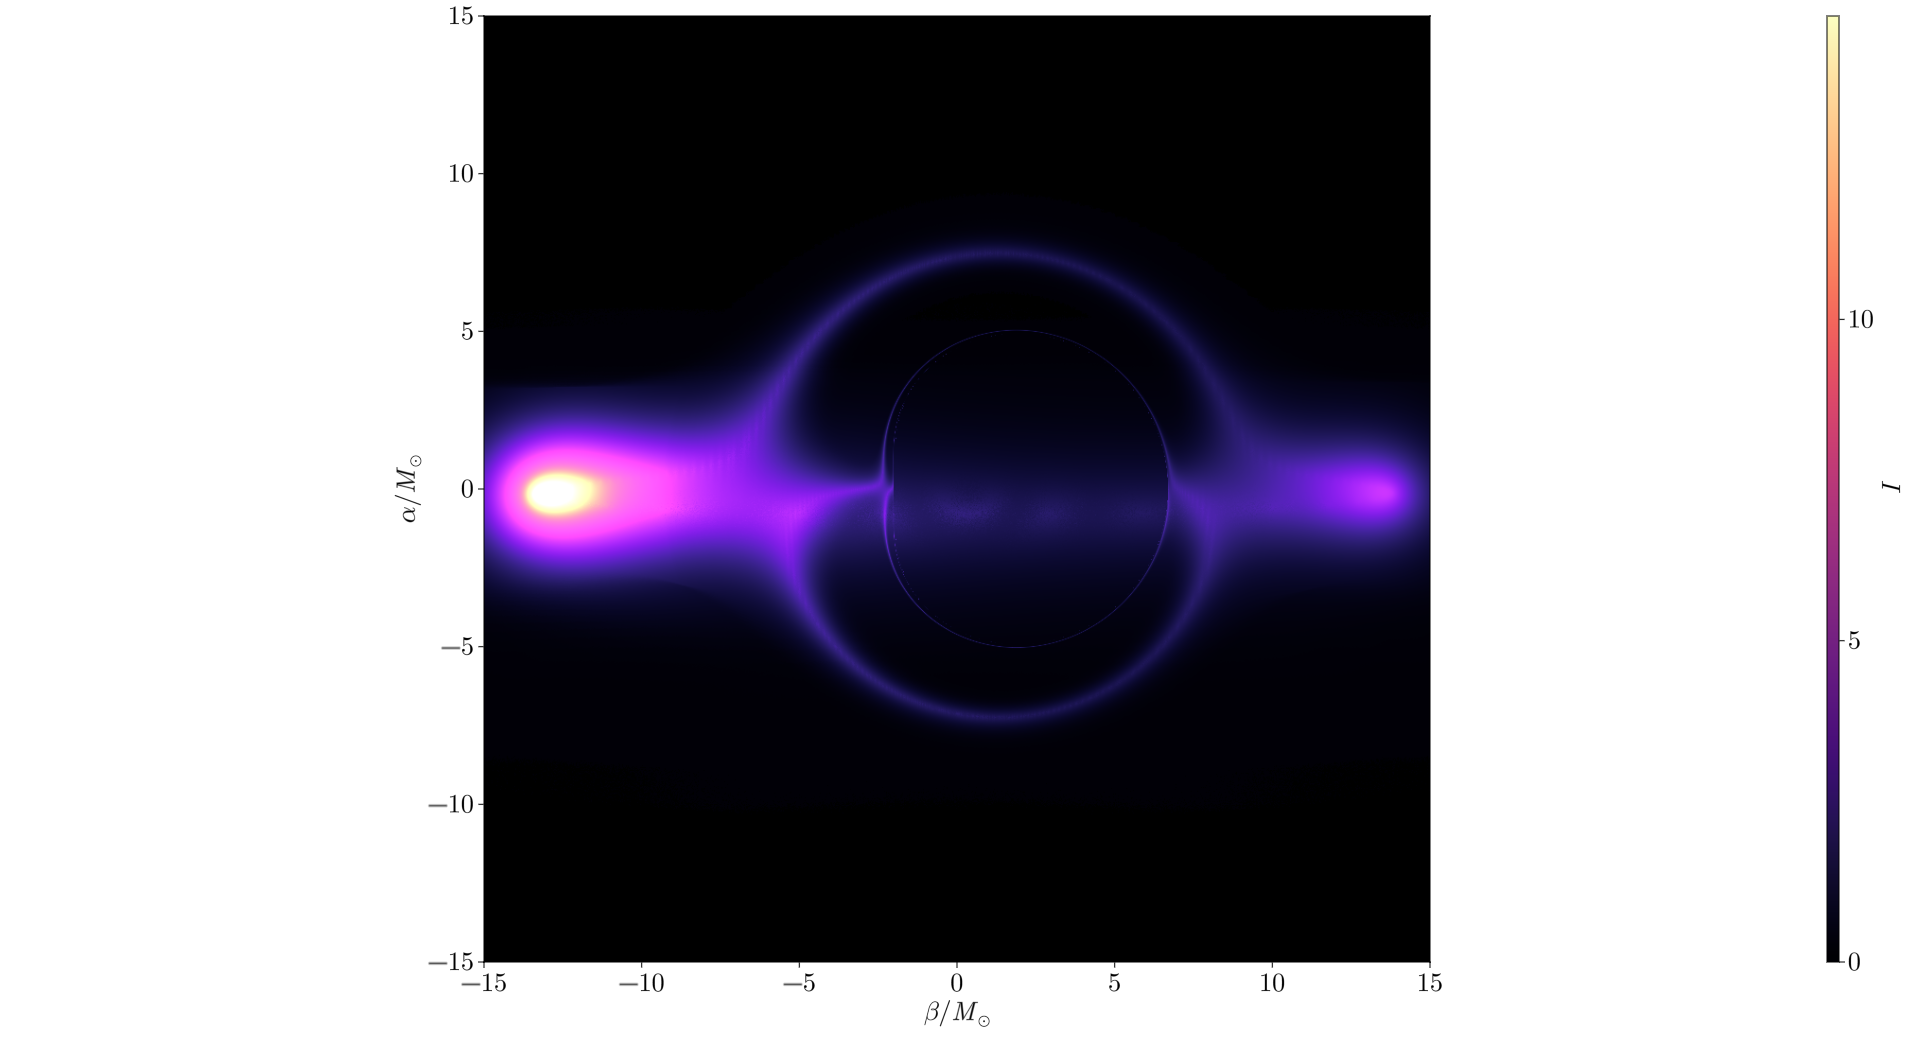
\includegraphics[width=1\textwidth]{figures/bh_shadow_1000x1000_a0998.png}
			\captionof{Kerr}{``D'' shape from frame-dragging ($a=0.998$).}
		\end{columns}
	\end{frame}
	
	\begin{frame}{Combined Scenario: Accretion Disk + Milky Way Background}
		\begin{itemize}
			\item The ultimate test of the framework: combining local astrophysical emission with a realistic celestial background.
			\item This synthetic image closely mimics the type of data analyzed by the Event Horizon Telescope (EHT).
		\end{itemize}
		\begin{figure}
			\centering
			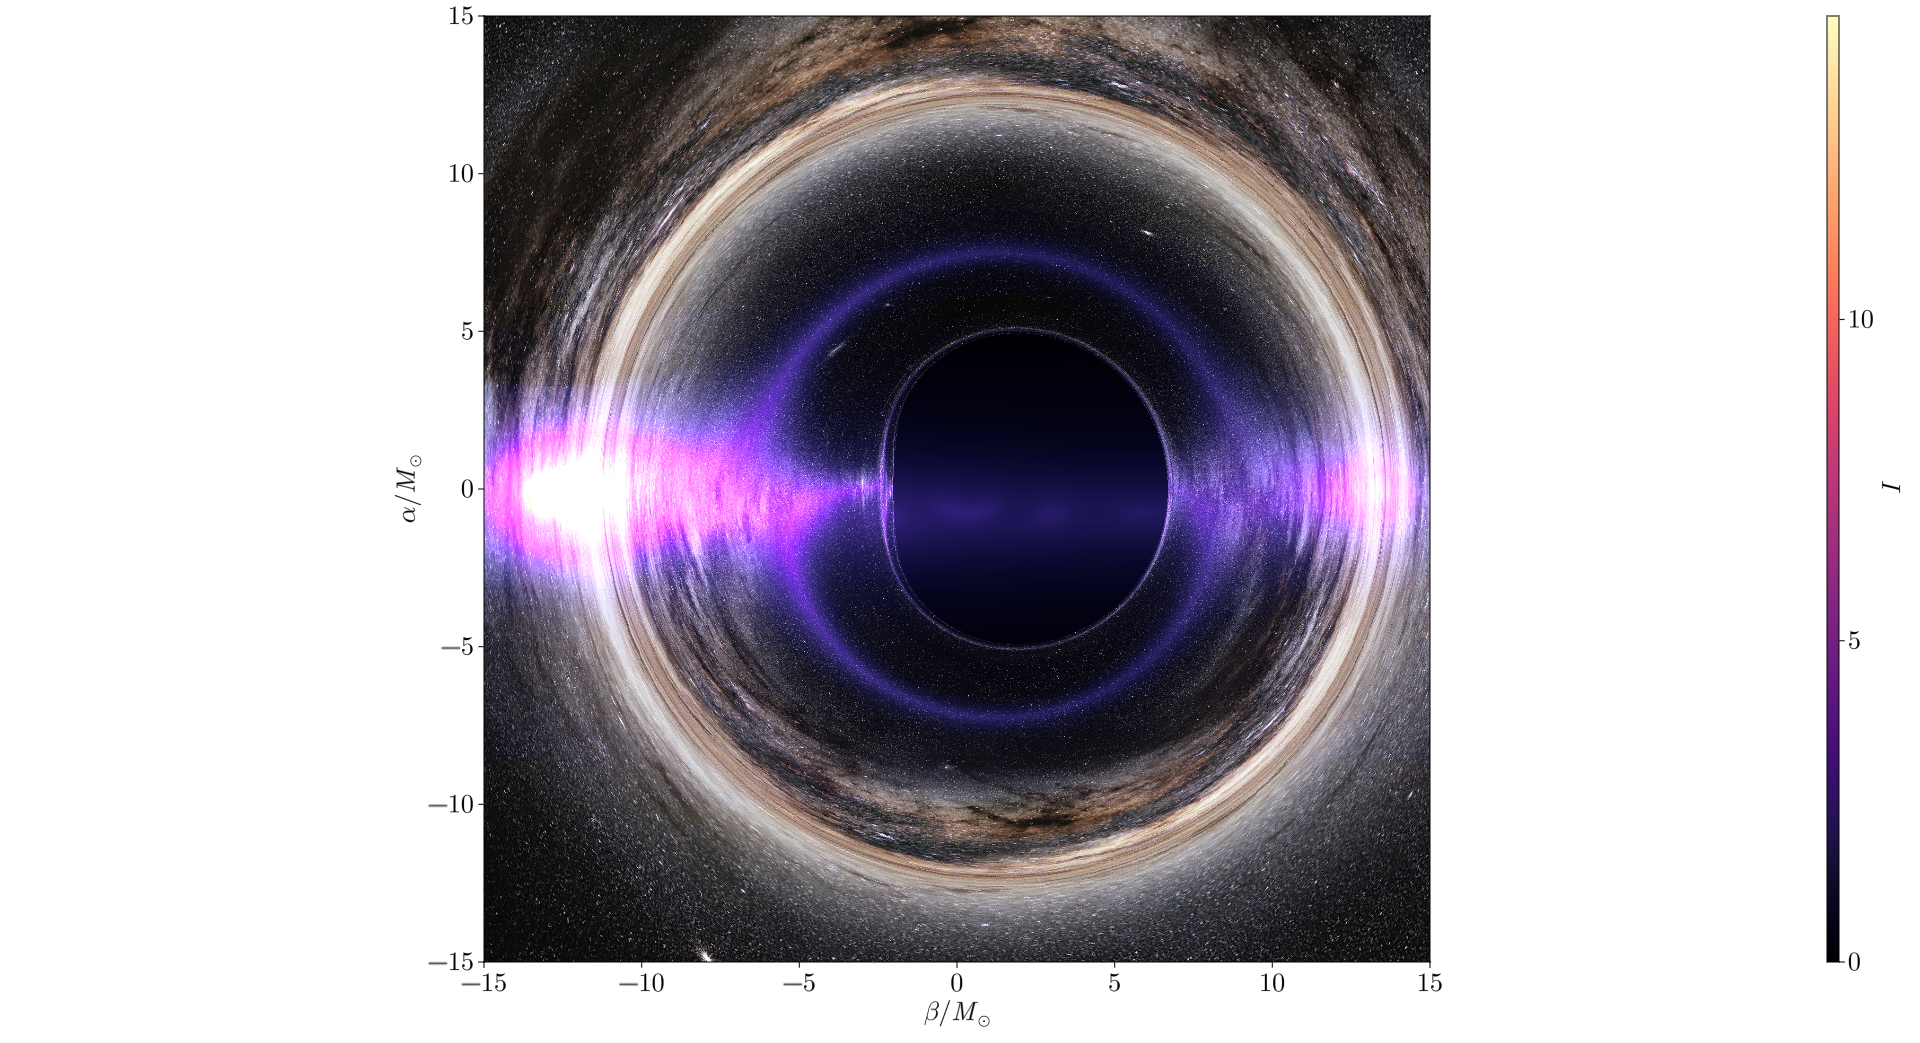
\includegraphics[width=0.68\textwidth]{figures/thin_disk_2000x2000_milky_way.png}
		\end{figure}
	\end{frame}
	
	\section{Conclusions}
	
	\begin{frame}{Conclusions}
		\begin{itemize}
			\item Developed a robust, metric-agnostic ray tracing framework in Julia.
			\item \textbf{Automatic Differentiation:} Exact metric derivatives, no truncation error.
			\item \textbf{Manifold Projection:} Invariants conserved to machine precision.
			\item Successfully resolved higher-order photon sub-rings and complex shadow morphologies.
			\item \textbf{High Performance:} On a standard 16-core laptop, the framework processes computationally demanding trajectories at an average rate of \textbf{1,000,000 rays in less than an hour}.
		\end{itemize}
	\end{frame}
	
	\begin{frame}
		\centering
		\Huge \textbf{Thank You!} \\
		\vspace{1cm}
		\Large Questions?
	\end{frame}
	
\end{document}
